% !TeX root = Main.tex

\section{Šíření ve volném prostředí} \label{sec:evlny_volne_prostredi}
\subsection{Popis elektromagnetického pole}
Elektromagnetickým vlněním je označováno šíření nestacionárního elektromagnetického pole. Jedná se o~vektorové pole, pro jehož obecný popis je potřeba znát následující čtveřici vektorů pole v~každém bodě prostoru\footnote{Vektory je v~této práci značeny tučným písmem.}\\ 

\begin{tabular}{lll}
$\vec E$ & $\unit{[V/m]}$ & intenzita elektrického pole,\\
$\vec D$ & $\unit{[C/m^{2}]}$ & elektrická indukce,\\
$\vec B$ & $\unit{[Wb/m^{2}],[T]}$ & magnetická indukce,\\
$\vec H$ & $\unit{[A/m]}$ & intenzita magnetického pole.\\
\end{tabular}\bigskip \\
Pro řešení pole ve vakuu nebo v~prostředí se známými materiálovými konstantami postačuje jakákoliv dvojice vektorů, kdy jeden je vektorem elektrického pole a druhý magnetického pole. To znamená, že libovolná dvojice z~variant $\vec E\vec B$, $\vec E\vec H$, $\vec D\vec H$ a~$\vec D\vec B$ je dostatečná po popis a řešení elektromagnetického pole.
Relace mezi vektory indukce a~intenzity příslušných polí popisují parametry prostředí 

\begin{equation}
	\vec D = \varepsilon\vec E = \varepsilon_{0}\varepsilon_{r}\vec E,
	\label{rce:D_epsE}
\end{equation}
\begin{equation}
	\vec B = \mu\vec H = \mu_{0}\mu_{r}\vec H,
	\label{rce:B_muH}
\end{equation}
\begin{equation}
	\vec J = \sigma\vec E.
	\label{rce:J_sigmaE}
\end{equation}
Rovnice (\ref{rce:J_sigmaE}) pro vektor proudové hustoty $\vec J$ v~prostředí s~volnými náboji je uvedena pro úplnost. V~tabulce \ref{tab:evlny_parametry_prostredi} se nachází popis a přehled možných materiálových parametrů prostředí včetně hodnot pro vakuum, které jsou odlišené indexem $0$. Naopak index $r$ v~rovnicích (\ref{rce:D_epsE}) a (\ref{rce:B_muH}) představuje označení relativních parametrů. V~závislosti na charakteru parametrů $\varepsilon$, $\mu$ a $\sigma$ se diferencuje prostředí dle několika vlastností, které jsou uvedeny v~tabulce \ref{tab:evlny_vlastnosti_prostredi}.

\begin{table}[!h]
\catcode`\-=12 
\begin{center}
  	\caption{Materiálové vlastnosti prostředí.}
  	\label{tab:evlny_parametry_prostredi}
\begin{tabular}{|lllp{1.5cm}l|}
	\hline
	permitivita		& $\varepsilon$	& $\unit{[F/m]}$ & 	& $\varepsilon_{0} = 8,854\cdot10^{-12}\unit{F/m} $\\
	
	permeabilita		& $\mu$		& $\unit{[H/m]}$ & 	& $\mu_{0} = 4\pi\cdot10^{-7}\unit{H/m}$\\
	
	měrná vodivost	& $\sigma$		& $\unit{[S/m]}$ & 	&\\
	\hline
\end{tabular}
\end{center}
\end{table}
\begin{table}[!h]
\catcode`\-=12 
\begin{center}
  	\caption{Dělení prostředí.}
  	\label{tab:evlny_vlastnosti_prostredi}
\begin{tabular}{|lp{0.3cm}|l|l|}
	\hline
	{\bf Linearita}									& & {\bf lineární}	& {\bf nelineární}	\\
	závislost $\varepsilon$, $\mu$ a $\sigma$ na veličinách pole 		& & nejsou závislé 	& závislé		\\ 
	\hline
	{\bf Homogennost}								& & {\bf homogenní}	& {\bf nehomogenní}	\\
	závislost $\varepsilon$, $\mu$ a $\sigma$ na prostorových souřadnicích 	& & nejsou závislé 	& závislé		\\
	\hline
	{\bf Izotropnost}								& & {\bf izotropní}	& {\bf anizotropní}	\\
	závislost $\varepsilon$, $\mu$ a $\sigma$ na směru vektorů veličin pole 	& & nejsou závislé 	& závislé		\\
	\hline
\end{tabular}
\end{center}
\end{table}

V~sousvislosti s~existencí materiálových parametrů určitého prostředí, ve kterém se elektromagnetická vlna pohybuje se, zavádí tzv. {\bf konstanta šíření} $\faz k$. Případně se označuje také jako {\bf vlnové číslo}. Je závislá na všech parametrech, které jsou v~tabulce \ref{tab:evlny_parametry_prostredi} a navíc také na frekvenci. Vyjadřuje se tedy následovně
\begin{displaymath}
	\faz k=\pm\sqrt{-\mj\omega\mu(\sigma+\mj\omega\varepsilon)}\unit{[m^{-1}]}.
\end{displaymath}
Jde o~komplexní parametr, který ovlivňuje charakter šíření elektromagnetické vlny. V~literatuře se dají nalézt odlišnost v~označení reálné a imaginární  části tohoto komplexního čísla. V~\cite{emp} a také v~zahraniční literatuře se užívá tento typ označení 
\begin{equation}
	\faz k~= \beta - \mj\alpha\unit{[m^{-1}]}.
	\label{rce:evlny_alphabeta}
\end{equation}
\begin{description}
\item[$\beta\unit{[dB/m]}$] - je {\bf fázová konstanta}, která určuje fázi šířící se harmonické vlny.
\item[$\alpha\unit{[rad/m]}$] - je označován {\bf měrný útlum}, vyjadřující změnu amlitudy vlny.
\end{description}

Dalším používaným parametrem, kterým je možné popsat dané prostředí, se označuje jako {\bf vlnová (charakteristická) impedance}  $\faz Z$. Lze jí definovat vztahem
\begin{displaymath}
	\faz Z~= \frac{\omega\mu}{\faz k} = \sqrt{\frac{\mj\omega\mu}{\mj\omega\varepsilon + \sigma}}\unit{[\Omega]}.
\end{displaymath}
Tato komplexní veličina popisuje relaci mezi intenzitami magnetického a elektrického pole v~daném prostředí
\begin{displaymath}
	\vecfaz E = \faz Z~\cdot \vecfaz H.
\end{displaymath}

\subsubsection*{Obecné vlnové rovnice diferenciálního charakteru}
 Podrobné odvození vlnových rovnic pro vektory pole $\vec E$ a $\vec B$, pro časově konstantní parametry prostředí, se nachází v~příloze \ref{sec:Odvozeni_CasPole}
\begin{equation}
	\nabla^{2}\vec E -\mu\sigma\frac{\partial\vec E}{\partial t}-\mu\varepsilon\frac{\partial^{2}\vec E}{\partial t^{2}} = \grad\frac{\rho}{\varepsilon}+\mu\frac{\partial\vec J_{\mathrm{ext}}}{\partial t},
	\label{rce:evlny_VlnR_ElPole}
\end{equation}
\begin{equation}
	\nabla^{2}\vec B -\mu\sigma\frac{\partial\vec B}{\partial t}-\mu\varepsilon\frac{\partial^{2}\vec B}{\partial t^{2}}= -\mu\,\rot\vec J_{\mathrm{ext}}.
	\label{rce:evlny_VlnR_MagPole}
\end{equation}

\subsection{Harmonické pole}
Vztahy (\ref{rce:evlny_VlnR_ElPole}) a (\ref{rce:evlny_VlnR_MagPole}), eventuálně vztahy uvedené v~příloze \ref{sec:Odvozeni_CasPole}, jsou platné pro obecnou časovou závislost zdrojových funkcí $\rho$ a $\vec J_{\mathrm{ext}}$. Pro řešení polí, především numerického charakteru, se využívají harmonické funkce ($\sin$ nebo $\cos$). Důvodem je komplikované až nemožné analytické řešení rovnic (\ref{rce:VlnR_ElPole}) a (\ref{rce:VlnR_MagPole}). Dále proto, že harmonické pole je možné snadno generovat a řada zařízení je založena na jejich využití. 

Pro časově proměnné harmonické pole je možné využít tzv. symbolicko - komplexní metodu. Její aplikace spočívá ve vyjádření daného vektoru pole pomocí fázoru vektoru. Ten totiž je závislý jen na prostorových souřadnicích a není časově proměnný.

Pokud se bude například intenzita elektrického pole $\vec E(x,y,z,t)$ měnit harmonicky v~závislosti na čase, můžeme jí zapsat takto
\begin{displaymath}
	\vec E(x,y,z,t) = \vec E(x,y,z)\sin\omega t.
\end{displaymath}
V~daném poli je možné vyjádřit vektor intenzity elektrického pole pomocí fázoru\footnote{Fázory jsou znázorněny podtržením písmene.} vektoru $\vecfaz E(x,y,z)$. Z~něj je možné vytvořit rotující fázor vektoru
\begin{equation}
	\vecfaz E_{\rot}(x,y,z) = \vecfaz E(x,y,z)\me^{\mj\omega t}.
	\label{rce:rotujici_fazor_vektoru}
\end{equation}
Nakonec lze určit časovou závislost vektoru pole pomocí vztahu
\begin{equation}
	\vec E(x,y,z,t) = \Im\Big\{ \vecfaz E_{\rot}(x,y,z)\Big\} = \Im\Big\{ \vecfaz E(x,y,z)\me^{\mj\omega t}\Big\}.
	\label{rce:casova_zavislost}
\end{equation}
Z~rovnice (\ref{rce:casova_zavislost}) vyplývají pro reprezentaci časově proměnného vektoru pole $\vec E(x,y,z,t)$ fázorem $\vecfaz E(x,y,z)$ následující vlastnosti pro obrazy derivace a integrálu. Ty jsou využity při odvození vlnových rovnic v~harmonickém prostředí v~příloze \ref{sec:Odvozeni_HarmPole}
\begin{displaymath}
	\frac{\partial \vec E(x,y,z,t)}{\partial t} \longrightarrow \mj\omega \vecfaz E(x,y,z),
\end{displaymath}
\begin{displaymath}
	\frac{\partial^{\mathrm{n}} \vec E(x,y,z,t)}{\partial t^{\mathrm{n}}} \longrightarrow (\mj\omega)^{n} \vecfaz E(x,y,z),
\end{displaymath}
\begin{displaymath}
	\int\!\!\vec E(x,y,z,t) \dif t \longrightarrow \frac{\vecfaz E(x,y,z)}{\mj\omega},
\end{displaymath}
\begin{displaymath}
	\int\underbrace{\ldots}_{\mathrm{n}}\int\!\!\vec E(x,y,z,t) \dif t \longrightarrow \frac{\vecfaz E(x,y,z)}{(\mj\omega)^{\mathrm{n}}}.
\end{displaymath}

\subsubsection*{Vlnové rovnice harmonického pole}
 Podrobné odvození vlnových rovnic harmonického pole pro vektory $\vec E$ a $\vec B$, pro konstantní parametry $\varepsilon$, $\mu$ a $\sigma$, se nachází v~příloze \ref{sec:Odvozeni_HarmPole}
\begin{equation}
	\nabla^{2}\vecfaz E +\faz k^{2}\vecfaz E = \grad\frac{\rho}{\varepsilon}+ \mj\omega\mu\vecfaz J_{\mathrm{ext}},
	\label{rce:evlny_VlnR_ElPole_harm} 
\end{equation}
\begin{equation}
	\nabla^{2}\vecfaz B +\faz k^{2}\vecfaz B = -\mu\,\rot\vecfaz J_{\mathrm{ext}}.
	\label{rce:evlny_VlnR_MagPole_harm} 
\end{equation}

\subsection{Rovinná homogenní vlna ve volném prostředí}
Princip šíření elektromagnetických vln ve volném prostředí lze z~několika důvodů demonstrovat na jednoduché variantě rovinné homogenní vlny, ačkoliv se vlny v~této formě téměř nevyskytují. Je to dáno především omezeností rozměrů zdroje elektromagnetického záření. Avšak pro dostatečnou vzdálenost od tohoto reálného zdroje lze podle obrázku \ref{obr:evlny_rovinna_vlna} aplikovat zjednodušení, při kterém se část sférické vlnopolochy ve volném prostředí považuje za rovinnou. Pro užití rovinných homogenních vln svědčí také nezanedbatelný fakt, že pomocí jejich součtu je možné sestavit libovolnou složitější obecnou vlnu. 

\begin{figure}[!h]
	\centering
	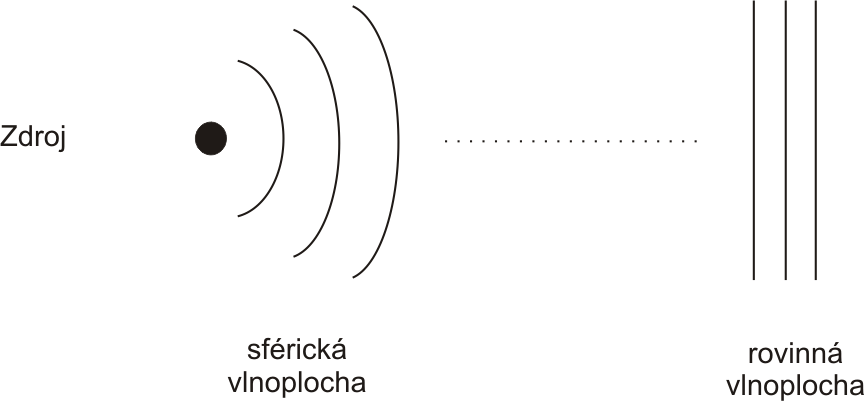
\includegraphics[width=9cm]{evlny_rovinna_vlna.png}
	\caption{Přiblížení rovinné vlny ve vzdáleném prostředí.}
	\label{obr:evlny_rovinna_vlna}
\end{figure}

V~teorii šíření elektromagnetických vln se dle \cite{emp} užívá řada pojmů, z~nichž některé jsou použity také v~této práci.
\begin{itemize}
\item {\bf Vlnoplocha} - Skupina bodů, které mají stejnou fázi a po jejich spojení tvoří geometrickou plochu vlny.
\item {\bf Volné neohraničené prostředí} - Prostor bez jakýkoliv překážek, kterými jsou předměty nebo objekty s~odlišnými materiálovými konstatami  $\varepsilon$, $\mu$ a $\sigma$ od prostředí, ve kterém se vlna šíří.
\item {\bf Homogenní vlna} - Označuje se také jako {\bf uniformní} a jedná se o~vlnu, která má na dané vlnoploše také konstatní amplitudu.
\end{itemize}

Pro analýzu libovolného obecného typu vln je nejprve potřeba zvolit vhodnou souřadnicovou soustavu. V~případě rovinné vlny se bude jednat o~kartézskou souřadnicovou soustavu. V~harmonickém poli bez vnějších zdrojů bude odvození vycházet z~homogenní Helmholtzovy rovnice (\ref{rce:VlnR_ElPole_harm_BezZdroju})
\begin{equation}
	\nabla^{2}\vecfaz E + \faz k^{2}\vecfaz E = 0.
	\label{rce:evlny_VlnR_ElPole_harm_BezZdroju}
\end{equation}
Aplikací operátoru $\nabla^{2}$ na vektor $\vecfaz E$ dostaneme opět vektor, který lze v~kartézské soustavě vyjádřit jako $\nabla^{2}\faz E_{x}\overrightarrow{\mathrm{i}} + \nabla^{2} \faz E_{y}\overrightarrow{\mathrm{j}} + \nabla^{2}\faz E_{z}\overrightarrow{\mathrm{k}}$. To způsobí rozpad vektorové rovnice (\ref{rce:evlny_VlnR_ElPole_harm_BezZdroju}) na skalární rovnice pro jednotlivé složky
\begin{displaymath}
	\nabla^{2} \faz E_{x} +\faz k^{2} \faz E_{x} = 0,
\end{displaymath}
\begin{displaymath}
	\nabla^{2} \faz E_{y} +\faz k^{2} \faz E_{y} = 0,
\end{displaymath}
\begin{displaymath}
	\nabla^{2} \faz E_{z} +\faz k^{2} \faz E_{z} = 0.
\end{displaymath}
Řešení této soustavy rovnic je možné provést {\bf metodou separace proměnných} nebo po zavedení určitých zjednodušujících podmínek jako {\bf jednorozměrnou diferenciální rovnici}, jak je naznačeno dále. Pro vysvětlení druhé varianty se nejprve tyto skalární vztahy rozepíšou následujícím způsobem
\begin{equation}
	\frac{\partial ^{2} \faz E_{x}}{\partial x^{2}} + \frac{\partial ^{2}\faz E_{x}}{\partial y^{2}} + \frac{\partial ^{2}\faz E_{x}}{\partial z^{2}} + \faz k^{2} \faz E_{x} = 0,
	\label{rce:evlny_skalarni1}
\end{equation}
\begin{equation}
	\frac{\partial ^{2} \faz E_{y}}{\partial x^{2}} + \frac{\partial ^{2} \faz E_{y}}{\partial y^{2}} + \frac{\partial ^{2} \faz E_{y}}{\partial z^{2}} + \faz k^{2} \faz E_{y} = 0,
	\label{rce:evlny_skalarni2}
\end{equation}
\begin{equation}
	\frac{\partial ^{2} \faz E_{z}}{\partial x^{2}} + \frac{\partial ^{2} \faz E_{z}}{\partial y^{2}} + \frac{\partial ^{2} \faz E_{z}}{\partial z^{2}} + \faz k^{2} \faz E_{z} = 0.
	\label{rce:evlny_skalarni3}	
\end{equation}
Je výhodné zvolit souřadnicovou soustavu tak, aby se vlna šířila ve směru jedné z~os. Poté bude platit, že vlnoplocha je rovina kolmá na tuto osu, tak jak je naznačeno na obrázku \ref{obr:evlny_vlnoplocha}. Současně uvažujeme pro zjednodušení vektor intenzity elektrického pole pouze ve směru osy $x$. Je možné jej také vyjádřit jako $\vecfaz E = \faz E_{x}\overrightarrow{\mathrm{i}}$.

\begin{figure}[!h]
	\centering
	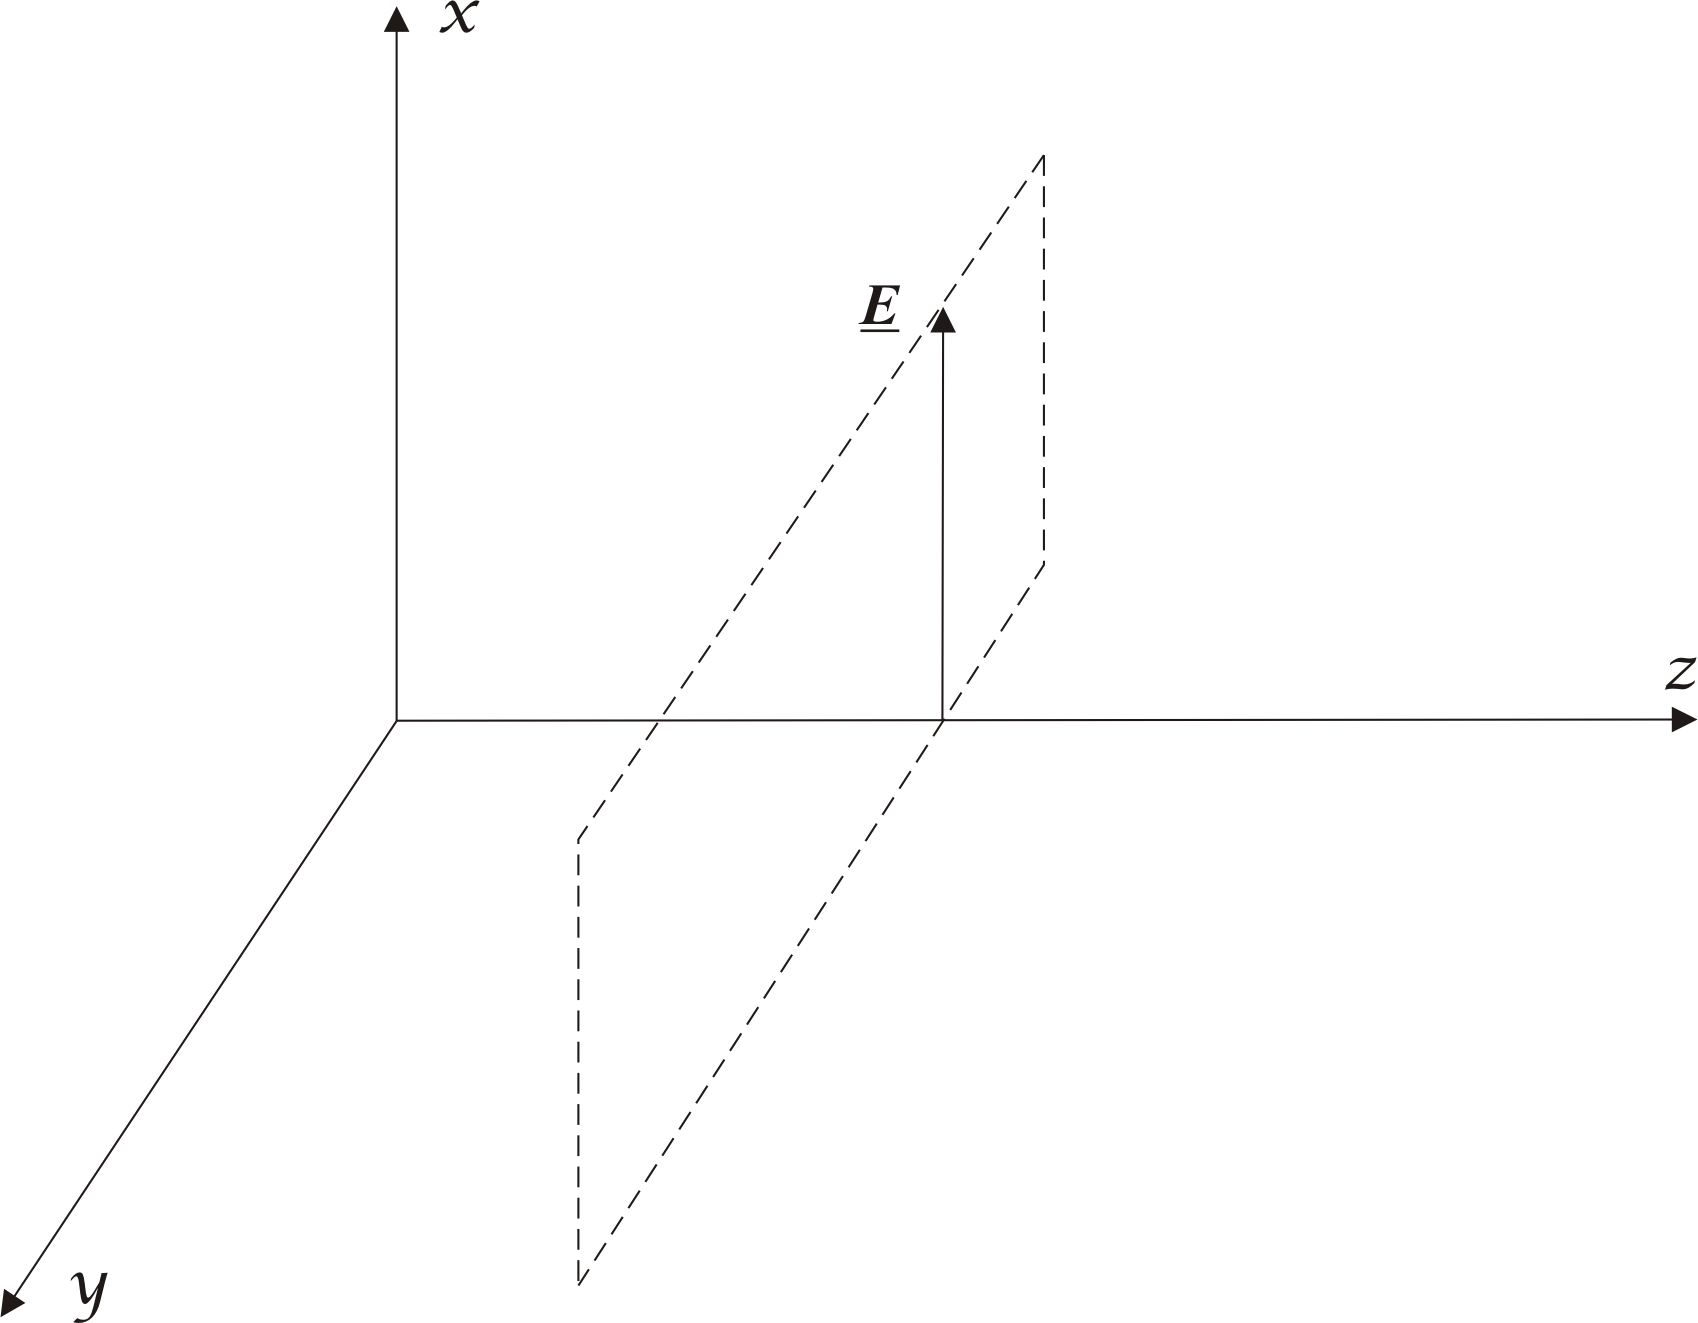
\includegraphics[width=10cm]{evlny_vlnoplocha.png}
	\caption{Vlnoplocha rovinné homogenní vlny. \cite{emp}}
	\label{obr:evlny_vlnoplocha}
\end{figure}

Z~výše uvedených úvah o~charakteru vln a jejich prostorového uspořádání vyplývají následující skutečnosti.
\begin{itemize*}
\item Konstantní velikost a fáze vektoru $\vecfaz E$ ve směru osy $x$, tzn. $\frac{\partial  \faz E_{x}}{\partial x}=0$ a $\frac{\partial \faz E_{x}}{\partial y}=0$.
\item Nulový vektor $\vecfaz E$ ve směru osy $y$, tzn. $ \faz E_{y} = 0$.
\item Nulový vektor $\vecfaz E$ ve směru osy $z$, tzn. $ \faz E_{z} = 0$.
\end{itemize*}
Pokud je aplikujeme na tři rozepsané skalární rovnice (\ref{rce:evlny_skalarni1}) až (\ref{rce:evlny_skalarni3}), dojde ke značnému matematickému zjenodušení. Rovnice (\ref{rce:evlny_skalarni2}) a (\ref{rce:evlny_skalarni3}) se úplně eliminují, u~rovnice (\ref{rce:evlny_skalarni1}) vypadnou první dva členy. Výsledná rovnice bude tak jednorozměrná obyčejná diferenciální druhého řádu ve tvaru
\begin{equation}
	\frac{\partial ^{2} \faz E_{x}}{\partial z^{2}} + \faz k^{2} \faz E_{x} = 0.
	\label{rce:evlny_skalarni}	
\end{equation}

\subsubsection*{Řešení rovnice rovinné homogenní vlny (\ref{rce:evlny_skalarni})}
Vzhledem k~jednoduchosti dané diferenciální rovnice můžeme rovnou předpokládat řešení v~následujícím tvaru
\begin{equation}
	\faz E_{x}(z) = \faz E_{0}^{+}\me^{\lambda_{1}z} +\faz E_{0}^{-}\me^{\lambda_{2}z},
	\label{rce:evlny_reseni1}	
\end{equation}
který představuje superpozici dvou funkcí. Výrazy $E_{0}^{+}$ a $E_{0}^{-}$ jsou komplexní konstanty dané složky vektoru. Parametry $\lambda_{1}$ a $\lambda_{2}$ se určují jako kořeny charakteristického polynomu dané diferenciální rovnice (\ref{rce:evlny_skalarni})
\begin{displaymath}
	\lambda^{2} + \faz k^{2}= 0,
\end{displaymath}
\begin{displaymath}
	\lambda_{1,2} = \pm \sqrt{-\faz k^{2}},
\end{displaymath}
\begin{displaymath}
	\lambda_{1} = -\mj\faz k~,\qquad \lambda_{2} = +\mj\faz k.
\end{displaymath}
Dosazením parametrů $\lambda_{1}$ a $\lambda_{2}$ do (\ref{rce:evlny_reseni1}) dostaneme vztah 
\begin{equation}
	\faz E_{x}(z) = \faz E_{0}^{+}\me^{-\mj\faz k~z} + \faz E_{0}^{-}\me^{\mj\faz k~z},
	\label{rce:evlny_reseni2}	
\end{equation}
který má jednoduchou fyzikální interpretaci. Podle obrázku \ref{obr:evlny_vlnoplocha} je zřejmé, že řešení vlnové rovnice je závislé pouze na souřadnici $z$ a vlnoplocha leží v~rovice $xy$. Takto vyjádřená vlna má pouze jeden stupeň volnosti a může se tedy šířit pouze v~kladném nebo záporném ve směru $z$.

První člen $ \faz E_{0}^{+}\me^{-\mj\faz k z}$ přestavuje funkci vlny šířící se v~kladném směru osy $z$ a označuje se jako {\bf postupná vlna}. Druhý člen $\faz E_{0}^{-}\me^{\mj\faz k z}$ popisuje funkci vlny pohybující se v~opačném směru, tzn. {\bf vlna odražená}.

Komplexní konstanty $\faz E_{0}^{+}$ a $\faz E_{0}^{-}$ je možné dále blíže rozepsat na část představující modul $E_{0\mathrm{mod}}$ a část pro reprezentaci fáze $\me^{j\varphi}$. S~využitím této vlastnosti upravíme rovnici (\ref{rce:evlny_reseni2}). Současně aplikujeme vztah konstanty šíření (\ref{rce:evlny_alphabeta}), tj. $\faz k = \beta - \mj\alpha$,
\begin{displaymath}
	\faz E_{x}(z) = E_{0\mathrm{mod}}^{+}\me^{\mj\varphi^{+}}\me^{-\mj(\beta - \mj\alpha)z} + E_{0\mathrm{mod}}^{-}\me^{\mj\varphi^{-}}\me^{\mj(\beta-\mj\alpha)z}.
\end{displaymath}
Pro určení časové závislosti se nejprve užije vztah (\ref{rce:rotujici_fazor_vektoru}) pro rotující fázor
\begin{displaymath}
	\faz E_{x\,\rot}(z) = E_{0\mathrm{mod}}^{+}\me^{\mj\varphi^{+}}\me^{-\mj\beta z}\me^{-\alpha z}\me^{\mj\omega t} + E_{0\mathrm{mod}}^{-}\me^{\mj\varphi^{-}}\me^{\mj\beta z}\me^{\alpha z}\me^{\mj\omega t}.
\end{displaymath}
Nakonec se podle předpisu (\ref{rce:casova_zavislost}) vyjádří okamžitá hodnota časově proměnné intenzity elektrického pole. Výsledný vztah reprezentuje okamžitou hodnotu postupné a odražené složky rovinné vlny v~harmonickém prostředí
\begin{equation}
	E_{x}(z,t) = E_{0mod}^{+}\me^{-\alpha z}\sin(\omega t - \beta z~+ \varphi^{+}) + E_{0mod}^{-}\me^{\alpha z}\sin(\omega t + \beta z~+ \varphi^{-}).
	\label{rce:evlny_postupna_odrazena}
\end{equation}

\begin{figure}[!h]
	\centering
	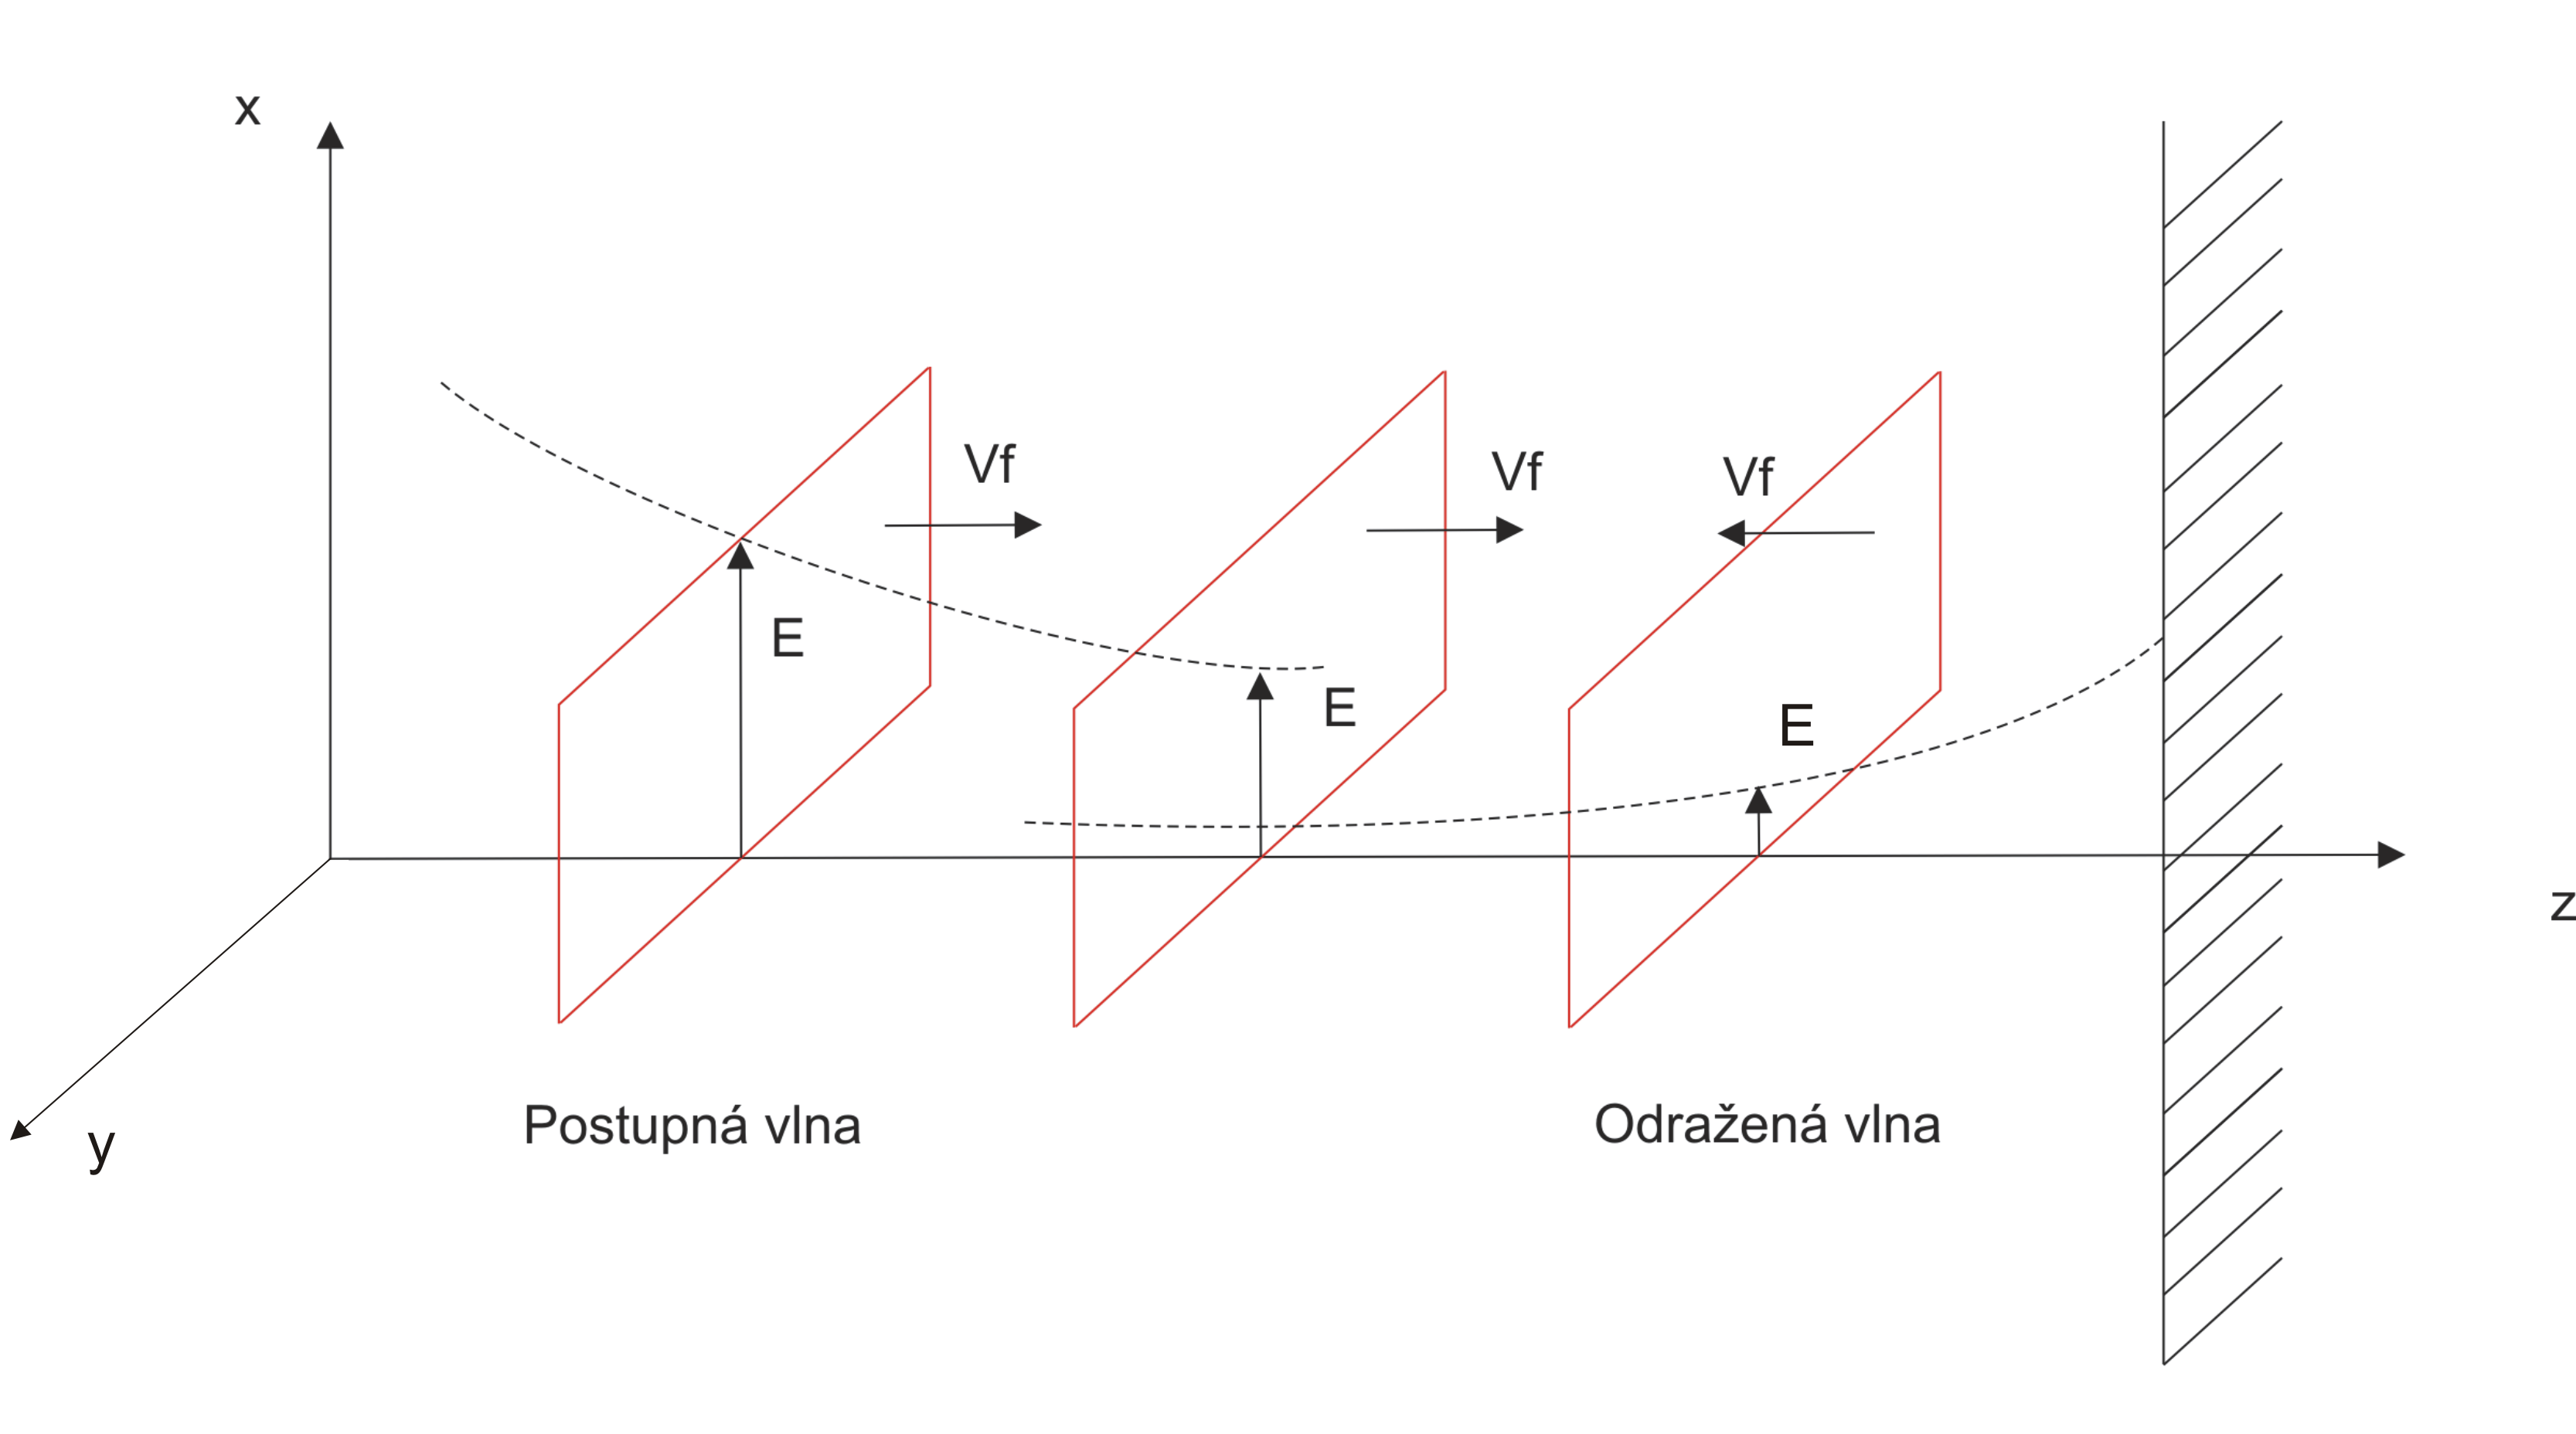
\includegraphics[width=14cm]{evlny_postupna_odrazena.png}
	\caption{Šíření postupné a odražené rovinné homogenní vlny dle (\ref{rce:evlny_postupna_odrazena}).}
	\label{obr:evlny_postupna_odrazena}
\end{figure}
\subsubsection*{Fázová rychlost vlny $v_{f}$}
Na obrázku \ref{obr:evlny_postupna_odrazena} je naznačen směr pohybu vln pomocí $v_{f}$. Rychlost, kterou se vlnoplocha ve směru osy $z$ pohybuje se označuje jako {\bf fázová rychlost vlny}. Výraz pro vyjádření odvodíme z~rovnice (\ref{rce:evlny_postupna_odrazena}). Vzhledem k~tomu, že vlnoplocha představuje rovinu bodů se stejnou fází, bude v~rovnici platit, $\omega t - \beta z + \varphi^{+} = \mathrm{konst.}$ pro postupnou vlnu. Podobně pro odraženou lze zapsat $\omega t + \beta z + \varphi^{-} = \mathrm{konst.}$

Pro odvození fázové rychlosti postupné vlny zderivujeme výraz $\omega t - \beta z + \varphi^{+} = \mathrm{konst.}$ podle času a následně upravíme
\begin{displaymath}
	\omega - \beta \frac{\dif z}{\dif t} = 0,
\end{displaymath}
\begin{displaymath}
	v_{f} = \frac{\dif z}{\dif t} = \frac{\omega}{\beta}\unit{[m/s]}.
\end{displaymath}
Analogickým odvozením z~výrazu pro odraženou vlnu  $\omega t + \beta z + \varphi^{-} = \mathrm{konst.}$ dostaneme vztah, který potvrzuje skutečnost, že odražená vlna se šíří podle osy $z$ v~opačném směru 
\begin{displaymath}
	v_{f} = - \frac{\omega}{\beta}\unit{[m/s]}.
\end{displaymath}

\subsubsection*{Obecné řešení rovnice (\ref{rce:evlny_VlnR_ElPole_harm_BezZdroju}) metodou separace proměnných}
V~řadě aplikacích není možné zavést pro řešení rovnice $\nabla^{2}\vecfaz E +\faz k^{2}\vecfaz E = 0$  zjednodušující předpoklady, vycházející z~obrázku \ref{obr:evlny_vlnoplocha}. Potom se rovnice řeší analyticky pomocí metody separace proměnných. Principem je nalézt řešení pro jednotlivé složky vektoru $\vecfaz E$ pomocí součinu tří funkcí, vždy jedné proměnné
\begin{equation}
	\faz E_{i}(x,y,z) = X(x)\cdot Y(y)\cdot Z(z)\qquad\mathrm{pro}\ i = x, y, z.
	\label{rce:evlny_obecne_xyz}
\end{equation}
Podrobné odvození je rozepsáno v~\cite[str. 50]{emp}. Řešení je ve tvaru součinů podle (\ref{rce:evlny_obecne_xyz})
\begin{equation}
	\faz E_{i}(x,y,z) = \big( \faz C_{1}\me^{\mj k_{x}x} +\faz C_{2}\me^{-\mj k_{x}x} \big)\big(\faz C_{3}\me^{\mj k_{y}y} + \faz C_{4}\me^{-\mj k_{y}y} \big)\big(\faz C_{5}\me^{\mj k_{z}z} + \faz C_{6}\me^{-\mj k_{z}z} \big).
	\label{rce:evlny_obecne_reseni}
\end{equation}
Všechny neznámé konstanty se určují na základě okrajových podmínek. Komplexní konstanty $\faz C_{1,\ldots,6}$ udávají amlitudu a fázi rovinných vln, složky konstanty šíření $k_{x}$, $k_{y}$ a $k_{z}$ určují směry šíření. Pomocí součtu určitého množství rovinných vln je tedy možné sestavit v~kartézské souřadnicové soustavě libovolnou vlnu.

\section{Rozhraní dvou prostředí} \label{sec:evlny_rozhrani_dvou_prostredi}
Podkapitola \ref{sec:evlny_volne_prostredi} se věnuje šíření elektromagnetických vln ve volném neohraničeném prostředí. Avšak pro reálnější popis je potřeba zvažovat také vliv překážek v~prostorově omezené oblasti. Důležitým stavebním kamenem pro formulování tohoto problém je, jak napovídá název podkapitoly, chování vln na rozhraní mezi odlišnými prostředími.

Při dopadu elektromagnetické vlny na materiálově odlišný objekt může dojít k~několika událostem, kterými jsou odraz, lom nebo prostup vlny. V~praxi se přirozeně nejedná striktně o~jeden typ chování. Častěji dojde k~jejich kombinaci, ve které mají jednotlivé složky určité zastoupení. Fyzikální vysvětlení spočívá v~existenci vodivých a posuvných proudů, které vzniknou právě při dopadu elektromagnetické vlny. Proudy představují zdroje pro vznik dalších vln, které se superponují k~původní vlně a ovlivní její vlastnosti. 

Matematický popis je možný u~některých příkladů po zavedení určitých zjednodušujících předpokladů. Vytvoření modelu pro obecný reálný případ nemusí být mnohdy vůbec proveditelné, neboť po dopadu vlny na překážku mohou nastat velmi komplikované procesy. Pro názornost je níže vysvětleno o~jaké procesy se může jednat v~jednoduchém případě rovinné homogenní vlny dopadající na rovinné rozhraní.

\subsection*{Chování rovinné vlny na rovinném rozhraní}
Tento případ by se z~hlediska matematického popisu dal nazvat jako téměř ideální. V~reálných variantách bude situace přirozeně jiná, ale i na tomto jednoduchém příkladu je možné popsat jevy, které nastanou po dopadu elektromagnetické vlny. 

Pro popis šíření se výhodně využívá dle \cite[str.47]{emp} tzv. vlnový vektor $\vec k_{vln}$. S~jeho pomocí lze snadno názorně popsat směry šíření vln na rozhraní. Vlnový vektor představuje to, v~jakém směru se šíří vlnoplocha. Dle obrázku \ref{obr:evlny_vlnovy_vektor} jej lze pomocí konstanty šíření $\faz k$ definovat
\begin{equation}
	\vec k_{vln} = \faz k~\vec n_{0} = k_{x}\overrightarrow{\mathrm{i}} + k_{y}\overrightarrow{\mathrm{j}} + k_{z}\overrightarrow{\mathrm{k}}.
	\label{rce:evlny_vlnovy_vektor}
\end{equation}

\begin{figure}[!h]
	\centering
	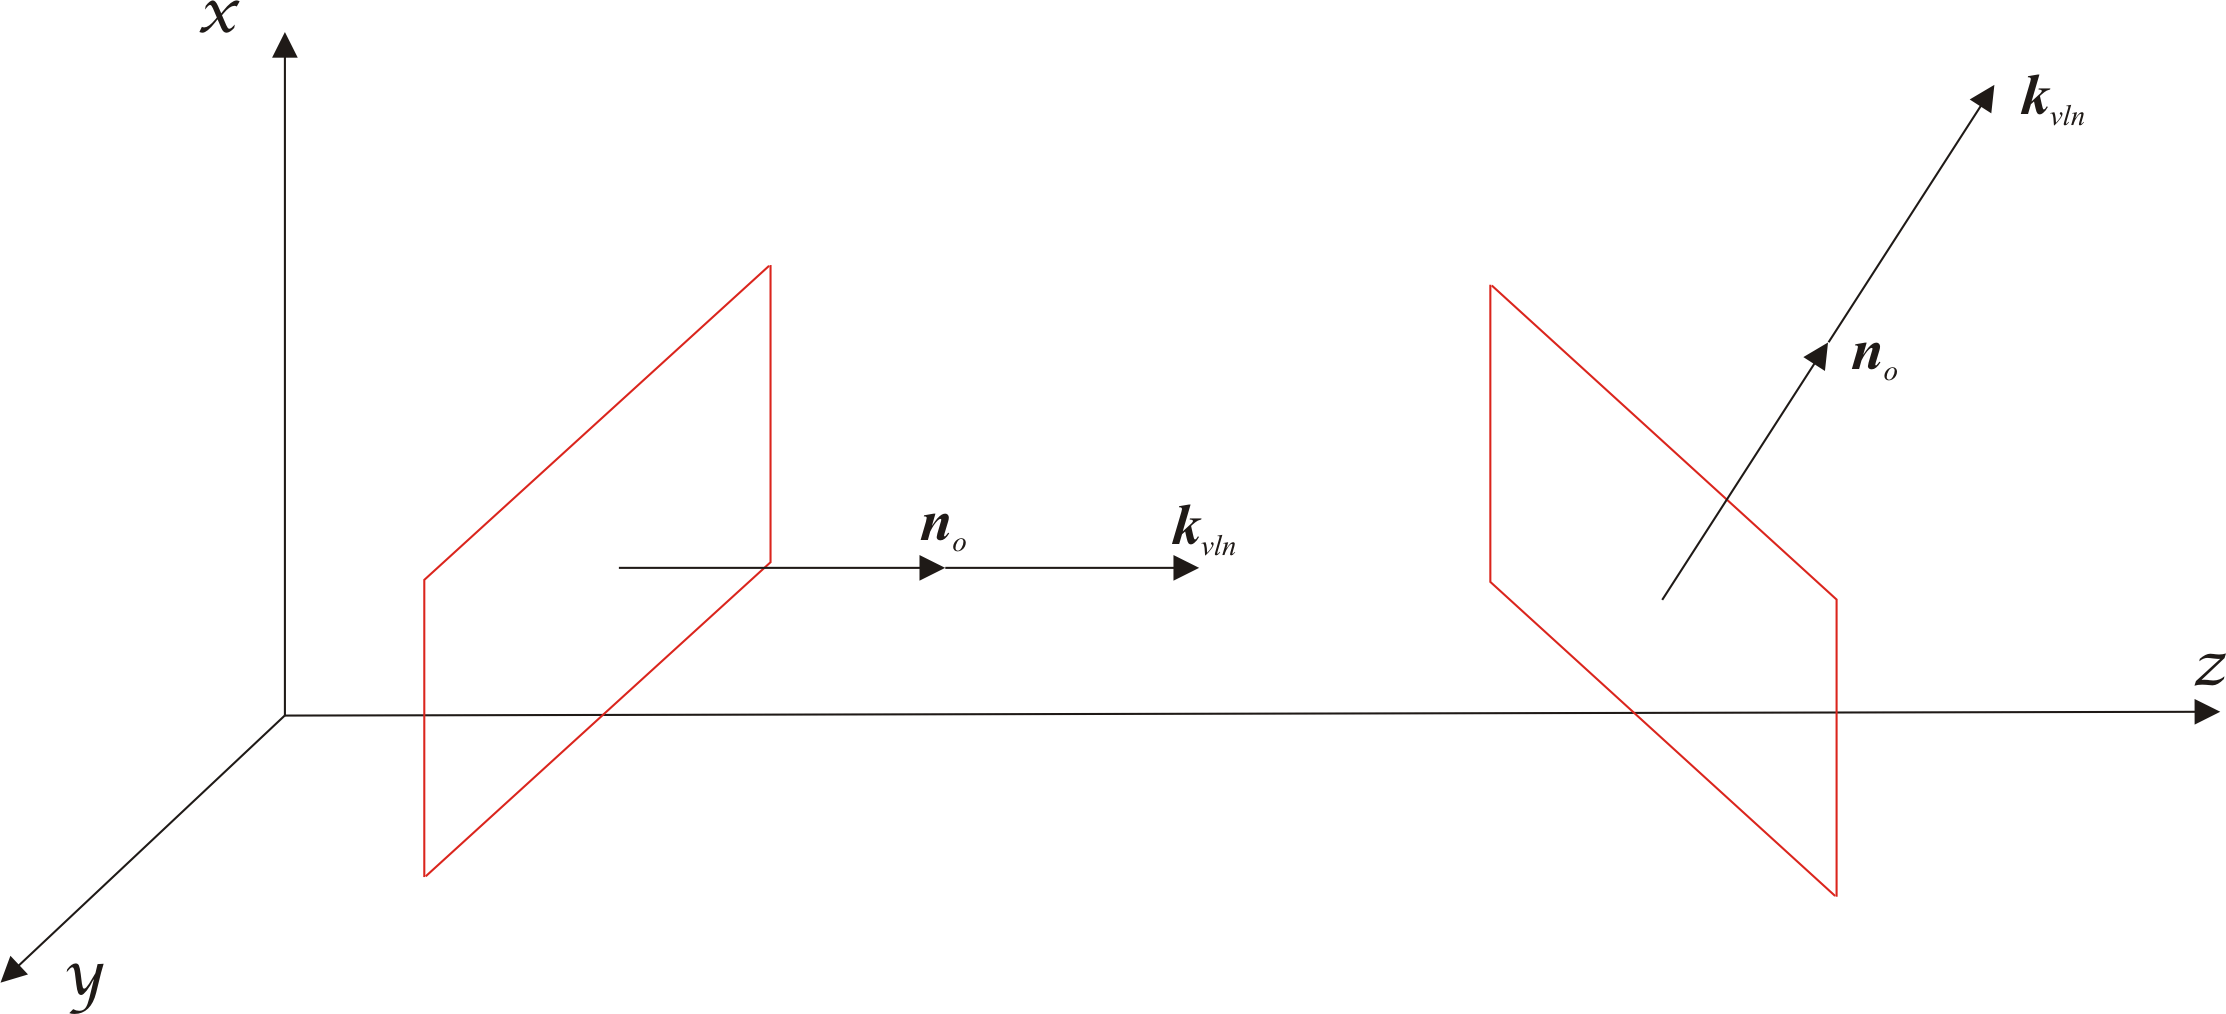
\includegraphics[width=13cm]{evlny_vlnovy_vektor.png}
	\caption{Definice vlnového vektoru v~kartézské soustavě souřadnic. \cite{emp}}
	\label{obr:evlny_vlnovy_vektor}
\end{figure}

Podle naznačené situace na obrázku \ref{obr:evlny_rovinne_rozhrani} je zřejmé, jak se může zachovat elektromagnetická vlna při dopadu pod obecným úhlem na rovinné rozhraní. Může dojít k~odrazu od rozhraní nebo průchodu do sousedícího prostředí, přičemž se se změní směr šíření (dojde k~lomu). Nejčastější bude případ, kdy se část vlny odrazí a současně část projde a bude se lámat. 

\begin{figure}[!h]
	\centering
	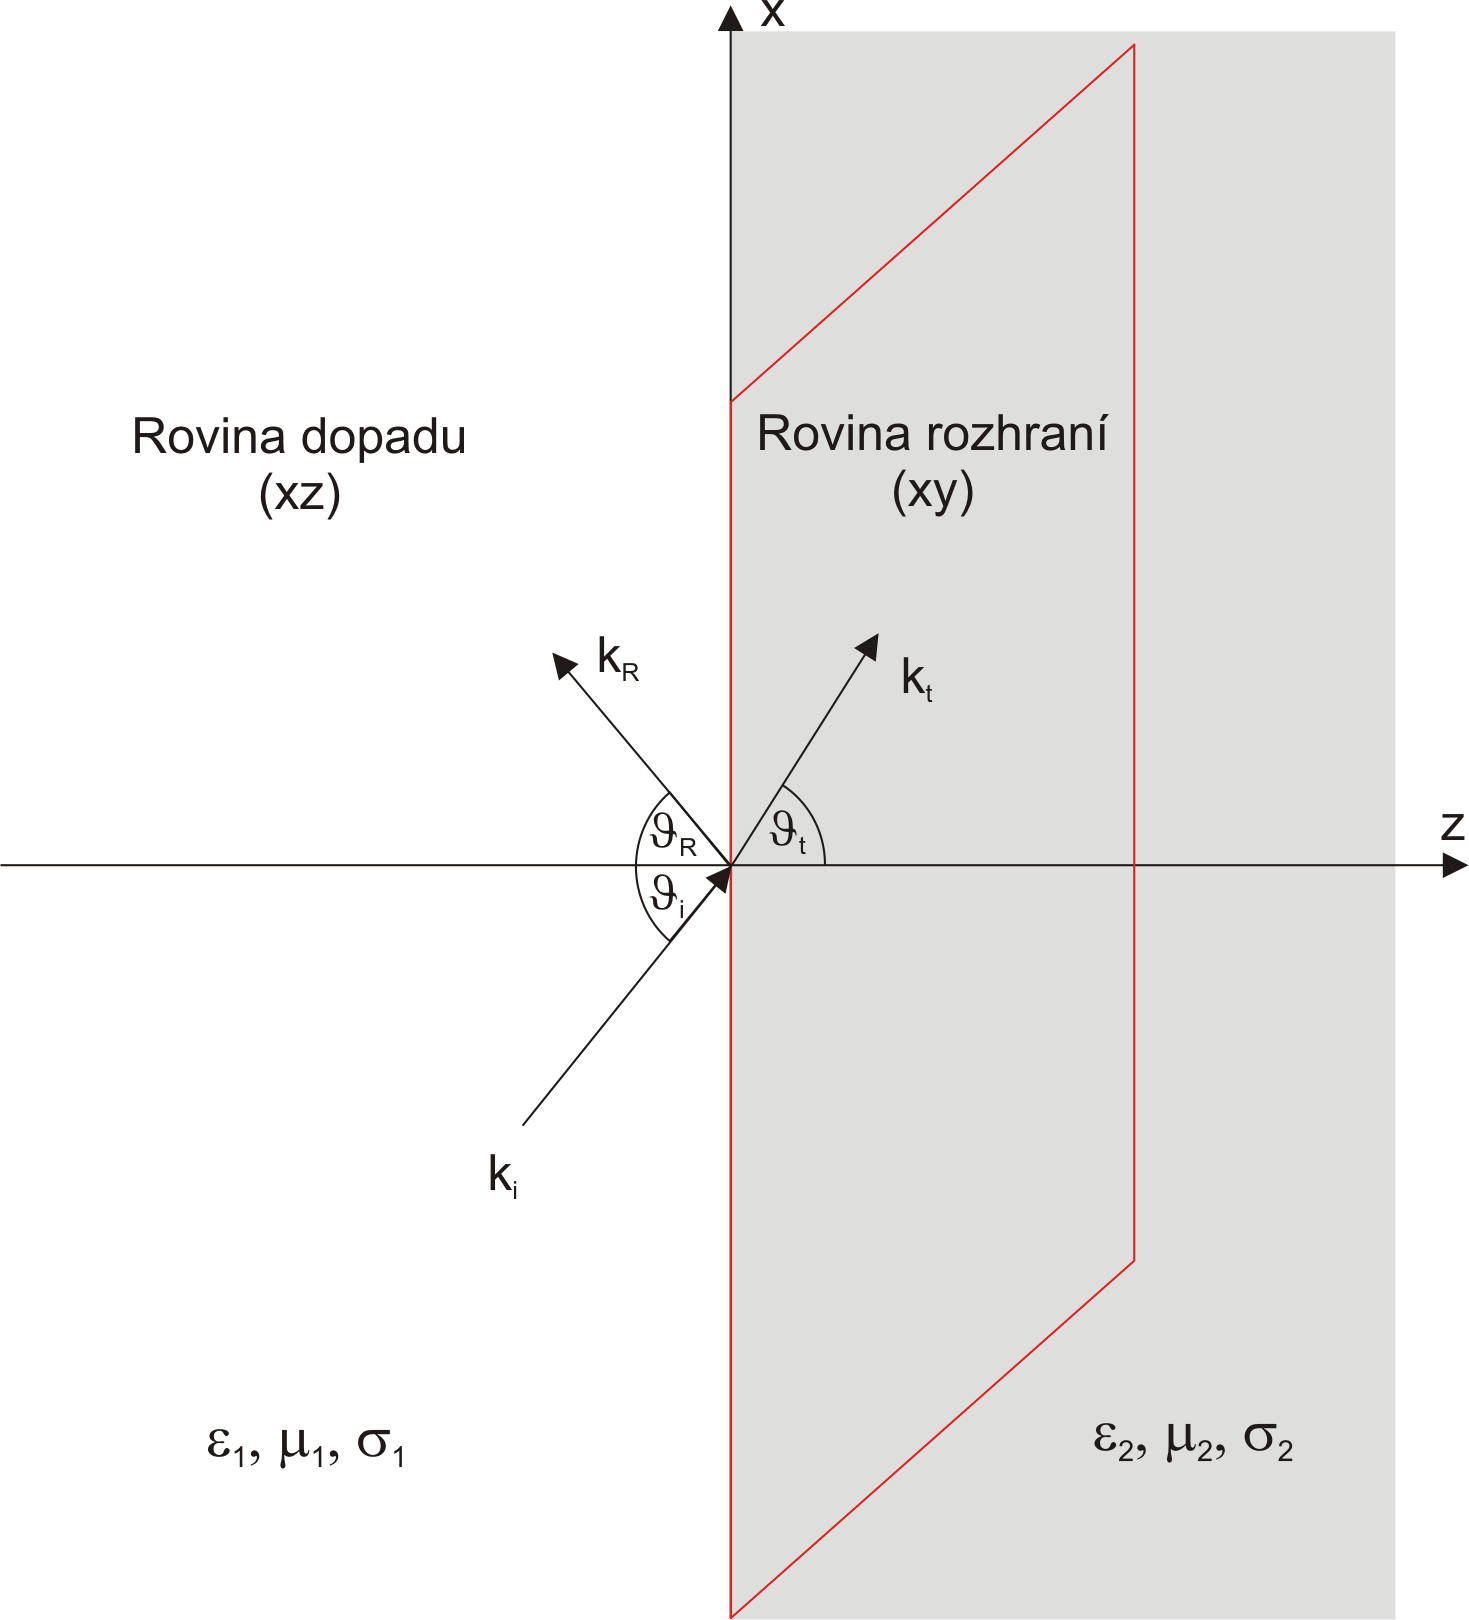
\includegraphics[width=8cm]{evlny_rovinne_rozhrani.png}
	\caption{Obecný dopad rovinné vlny na rozhraní s~využitím vlnového vektoru.}
	\label{obr:evlny_rovinne_rozhrani}
\end{figure}

Jak je navíc z~obrázku patrné, hranice mezi prostředími leží v~rovině $xy$. Označuje se jako {\bf rovina rozhraní}. Jednotlivé prostředí se liší materiálovými konstantami $\varepsilon$, $\mu$ a $\sigma$. Vlna se šíří ve směru osy $z$, tak jak bylo uvažováno již v~podkapitole \ref{sec:evlny_volne_prostredi}. Dopadá na rovinu rozhraní pod úhlem $\vartheta_{i}$ (z~anglického \uv{incident wave}). Část vlny se odráží pod úhlem $\vartheta_{r}$ (\uv{ref{l}ected}) a část proniká pod úhlem $\vartheta_{t}$ (\uv{transmitted}). Vlnové vektory všech tří variant jsou vyznačeny na obrázku \ref{obr:evlny_rovinne_rozhrani}. Rovina, ve které leží vektor dopadající vlny $k_{i}$, tvořená osami $xz$, se značí jako {\bf rovina dopadu}.

Splnění podmínek na rozhraní pro tečné složky vektorů $\vec E$ a $\vec H$ nastane, když jsou shodné $x$-ové složky vlnových vektorů, tj. $k_{i\,x} = k_{r\,x} = k_{t\,x}$. Dle obrázku \ref{obr:evlny_rovinne_rozhrani} je patrné, že s~využitím naznačených úhlů, lze zapsat
\begin{displaymath}
	\vec k_{i}\sin\vartheta_{i} = \vec k_{r}\sin\vartheta_{r} = \vec k_{t}\sin\vartheta_{t}.
\end{displaymath}
Vzhledem k~shodnosti prostředí, ve kterém se nachází postupná a odražená vlna, je možné s~využitím vztahu (\ref{rce:evlny_vlnovy_vektor}) definovat $\faz k_{1} = \vec k_{i} = \vec k_{r}$. Obdobně pro druhé prostředí platí $\faz k_{2} = \vec k_{t}$. Vyjádřený vztah (\ref{rce:evlny_snell_odvozeni}) je výchozím pro Snellovy zákony
\begin{equation}
	\faz k_{1}\sin\vartheta_{i} = \faz k_{1}\sin\vartheta_{r} = \faz k_{2}\sin\vartheta_{t}.
	\label{rce:evlny_snell_odvozeni}
\end{equation}
\begin{itemize}
\item {\bf Zákon odrazu} - Platí pro dopadající a odraženou elektromagnetickou vlnu. Lze jej také ústně interpretovat jako: \uv{Úhel odrazu se rovná úhlu dopadu}
\end{itemize}
\begin{displaymath}
	\faz k_{1}\sin\vartheta_{i} = \faz k_{1}\sin\vartheta_{r},
\end{displaymath}
\begin{equation}
	\vartheta_{i} = \vartheta_{r}.
	\label{rce:evlny_zakon_odrazu}
\end{equation}
\begin{itemize}
\item {\bf Zákon lomu} - Platí pro dopadající vlnu a pro vlnu pronikající do druhého prostředí
\end{itemize}
\begin{displaymath}
	\faz k_{1}\sin\vartheta_{i} = \faz k_{2}\sin\vartheta_{t},
\end{displaymath}
\begin{equation}
	\frac{\faz k_{2}}{\faz k_{1}} = \frac{\sin\vartheta_{i}}{\sin\vartheta_{t}}.
	\label{rce:evlny_zakon_lomu}
\end{equation}

\subsection{Kolmý dopad rovinné vlny na rozhraní} \label{subsec:kolmy_dopad}
V~konkrétním případě, dle obrázku \ref{obr:evlny_dielektricke_rozhrani}, je naznačen dopad rovinné homogenní vlny na rovinné rozhraní mezi dvěma prostředími. Ty jsou popsány obecně materiálovými parametry $\varepsilon_{1,2}$, $\mu_{1,2}$ a $\sigma_{1,2}$. Z~nich je možné vztahem $\faz Z=\sqrt{\frac{\mj\omega\mu}{\mj\omega\varepsilon + \sigma}}$ vyjádřit vlnové impedance pro jednotlivé prostředí.

\begin{figure}[!h]
	\centering
	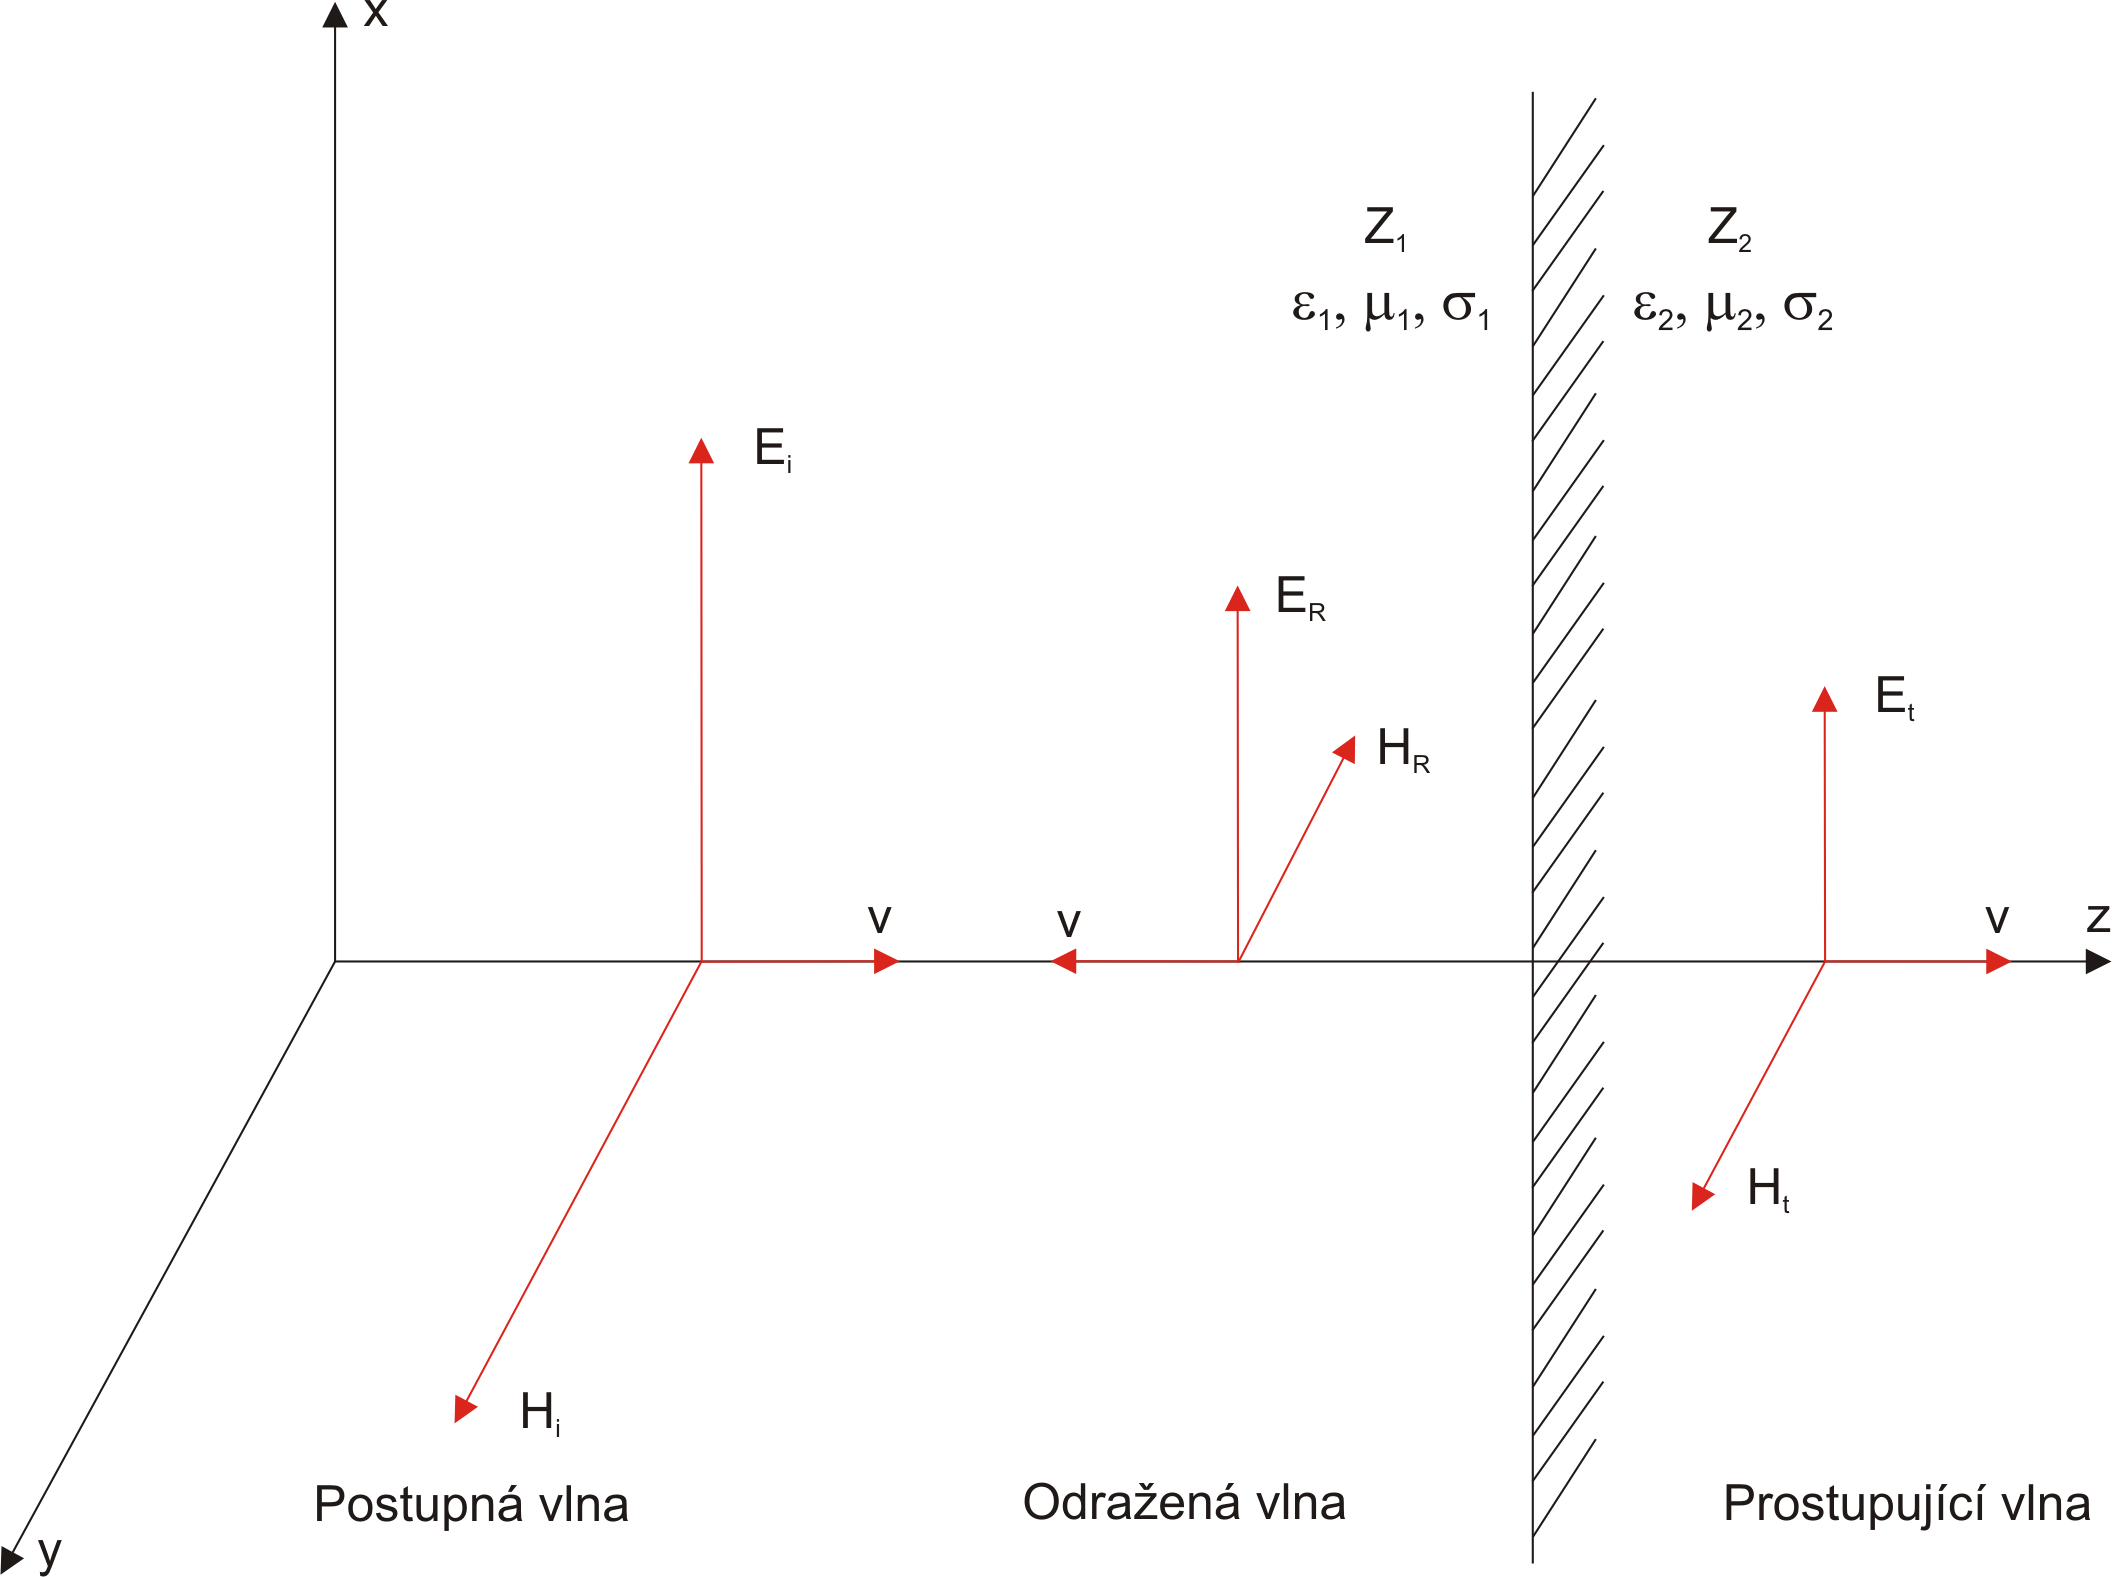
\includegraphics[width=13.5cm]{evlny_dielektricke_rozhrani.png}
	\caption{Kolmý dopad rovinné vlny rozhraní mezi dielektriky.}
	\label{obr:evlny_dielektricke_rozhrani}
\end{figure}

Vlny, které dopadají na rozhraní, lze zapsat vztahy pro vektory intezity elektrického pole $\vecfaz E_{i}$ a magnetického $\vecfaz H_{i}$ v~závislosti na souřadnici $z$
\begin{displaymath}
	\vecfaz E_{i}(z) = \faz E_{i0}\me^{-\mj\faz k_{1}z}\overrightarrow{\mathrm{i}},
\end{displaymath}
\begin{displaymath}
	\vecfaz H_{i}(z) = \frac{\faz E_{i0}}{\faz Z_{1}}\me^{-\mj\faz k_{1}z}\overrightarrow{\mathrm{j}}.
\end{displaymath}
Pro odraženou vlnu platí
\begin{displaymath}
	\vecfaz E_{r}(z) = \faz E_{r0}\me^{\mj\faz k_{1}z}\overrightarrow{\mathrm{i}},
\end{displaymath}
\begin{displaymath}
	\vecfaz H_{r}(z) = - \frac{\faz E_{r0}}{\faz Z_{1}}\me^{\mj\faz k_{1}z}\overrightarrow{\mathrm{j}},
\end{displaymath}
a~nakonec pro prostupující vlnu
\begin{displaymath}
	\vecfaz E_{t}(z) = \faz E_{t0}\me^{-\mj\faz k_{2}z}\overrightarrow{\mathrm{i}},
\end{displaymath}
\begin{displaymath}
	\vecfaz H_{t}(z) = \frac{\faz E_{t0}}{\faz Z_{2}}\me^{-\mj\faz k_{2}z}\overrightarrow{\mathrm{j}}.
\end{displaymath}
Podle podmínek na rozhraní ($z = 0$) se určí závislosti komplexních amplitud. Vychází se z~uvedených vztahů pro dopadající, odraženou a pronikající vlnu.
Pro vektor intenzity elektrického pole platí
\begin{displaymath}
	\vecfaz E_{i}(0) + \vecfaz E_{r}(0)  = \vecfaz E_{t}(0),
\end{displaymath}
\begin{displaymath}
	 \faz E_{i0}\me^{-j\faz k_{1}0}\overrightarrow{\vec{i}} + \faz E_{r0}\me^{j\faz k_{1}0}\overrightarrow{\mathrm{i}}  = \faz E_{t0}\me^{-j\faz k_{2}0}\overrightarrow{\mathrm{i}},
\end{displaymath}
\begin{equation}
	\faz E_{i0} + \faz E_{r0}  = \faz E_{t0}.
	\label{rce:evlny_rozhrani_E}
\end{equation}
Pro vektor intenzity magnetického pole na daném rozhraní se jedná o~analogické odvození, tj. $\vecfaz H_{i}(0) + \vecfaz H_{r}(0)  = \vecfaz H_{t}(0)$, čímž dostaneme
\begin{equation}
	\frac{\faz E_{i0}-\faz E_{r0}}{\faz Z_{1}} = \frac{\faz E_{t0}}{\faz Z_{2}}.
	\label{rce:evlny_rozhrani_H}
\end{equation}
Za $\faz E_{t0}$ se dosadí z~rovnice (\ref{rce:evlny_rozhrani_E}) do (\ref{rce:evlny_rozhrani_H}) . Dostaneme závislost $\faz E_{r0}$ na $\faz E_{i0}$, na jejíž základě se dle \cite{emp} definuje {\bf činitel odrazu (reflexe)}  $\faz R = \frac{\faz E_{r0}}{\faz E_{i0}}\unit{[-]}$
\begin{displaymath}
	\frac{\faz E_{i0}-\faz E_{r0}}{\faz Z_{1}} = \frac{\faz E_{i0} + \faz E_{r0}}{\faz Z_{2}},
\end{displaymath}
\begin{displaymath}
	\faz E_{r0}\Big( \frac{1}{\faz Z_{1}} + \frac{1}{\faz Z_{2}} \Big) = \faz E_{i0}\Big( \frac{1}{\faz Z_{1}} - \frac{1}{\faz Z_{2}} \Big),
\end{displaymath}
\begin{equation}
	\faz E_{r0} = \faz E_{i0} \frac{\faz Z_{2}-\faz Z_{1}}{\faz Z_{1}+\faz Z_{2}}.
	\label{rce:evlny_cin_odrazu_odvozeni}
\end{equation}
Z~rovnice (\ref{rce:evlny_cin_odrazu_odvozeni}) je patrný činitel odrazu
\begin{equation}
	\faz R = \frac{\faz Z_{2}-\faz Z_{1}}{\faz Z_{1}+\faz Z_{2}}.
	\label{rce:evlny_cin_odrazu}
\end{equation}
 Pokud chceme vyjádřit závislost $\faz E_{t0}$ na $\faz E_{i0}$ dosadíme z~(\ref{rce:evlny_rozhrani_E}) do (\ref{rce:evlny_rozhrani_H}) za $\faz E_{r0}$. Následně se určuje {\bf činitel prostupu (transmise)}  $\faz T = \frac{\faz E_{t0}}{\faz E_{i0}}\unit{[-]}$ 
\begin{displaymath}
	\frac{\faz E_{i0}-\faz E_{t0}+\faz E_{i0}}{\faz Z_{1}} = \frac{\faz E_{t0}}{\faz Z_{2}},
\end{displaymath}
\begin{displaymath}
	\faz E_{t0} \frac{\faz Z_{1}+\faz Z_{2}}{\faz Z_{1}\faz Z_{2}} = \faz E_{i0} \frac{2}{\faz Z_{1}}.
\end{displaymath}
\begin{equation}
	\faz E_{t0} = \faz E_{i0} \frac{2\faz Z_{2}}{\faz Z_{1}+\faz Z_{2}}.
	\label{rce:evlny_cin_prostupu_odvozeni}
\end{equation}
V~(\ref{rce:evlny_cin_prostupu_odvozeni}) je opět zřejmý činitel prostupu
\begin{equation}
	\faz T = \frac{2\faz Z_{2}}{\faz Z_{1}+\faz Z_{2}}.
	\label{rce:evlny_cin_prostupu}
\end{equation}
Vztahy pro oba činitele (\ref{rce:evlny_cin_prostupu}) a (\ref{rce:evlny_cin_odrazu}) jsou na sobě závislé a řídí se vztahem $1 + \faz R = \faz T$.

\subsection{Dopad rovinné vlny pod obecným úhlem}
Při analýze chování dopadající rovinné vlny pod jiným úhlem, než aby se jednalo o~kolmý dopad, se rozlišuje, zda se jedná o~kolmou (horizontální) nebo rovnoběžnou (vertikální) polarizaci vlny. Orientace se určuje podle vektoru intenzity elektrického pole $\vecfaz E$.
\subsubsection*{Kolmá polarizace}
Vektor $\vecfaz E$ je v~tomto případě kolmý na rovinu dopadu, tj. $xz$, podle obrázku \ref{obr:evlny_kolma_polarizace}.
\begin{figure}[!h]
	\centering
	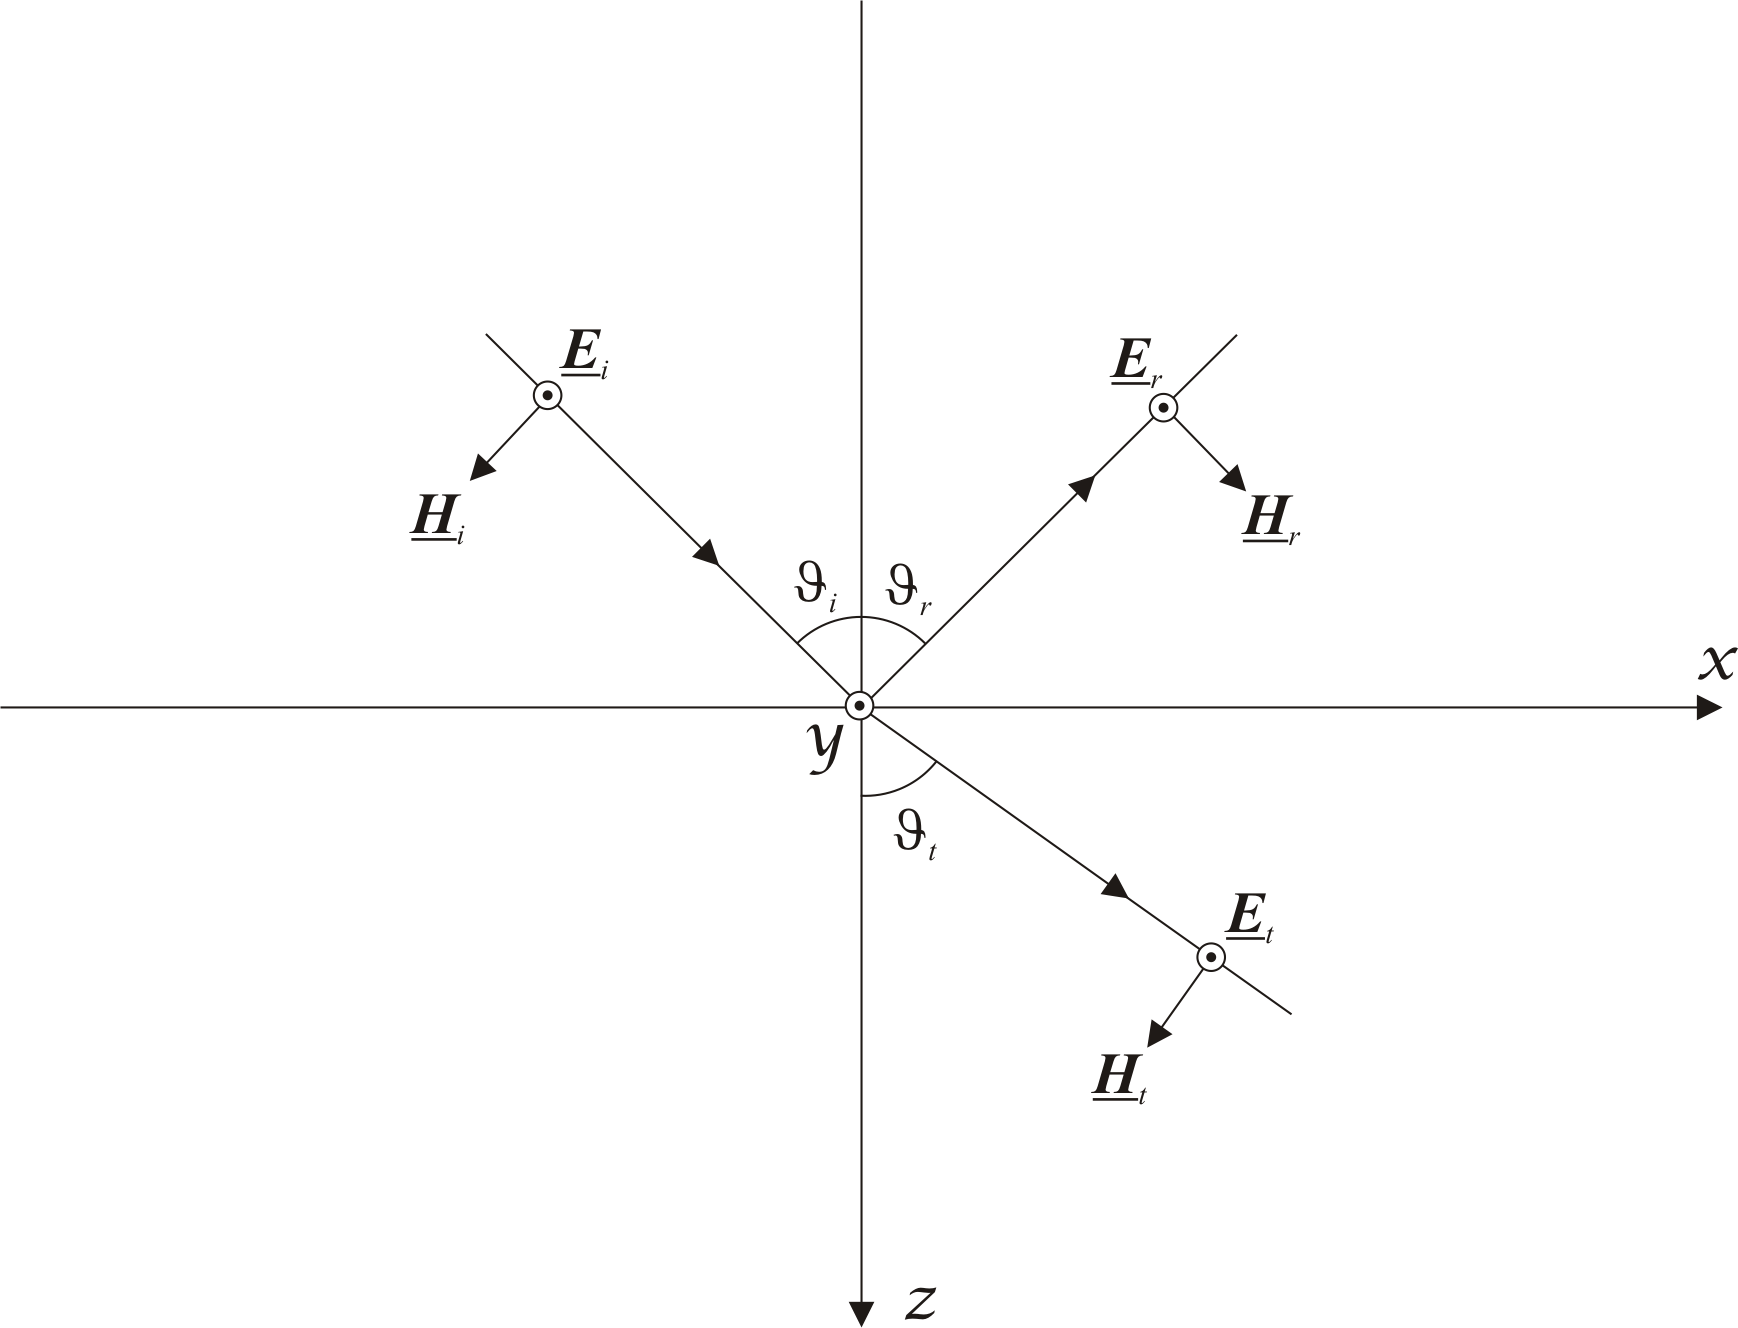
\includegraphics[width=11cm]{evlny_kolma_polarizace.png}
	\caption{Kolmá polarizace rovinné vlny. \cite{emp}}
	\label{obr:evlny_kolma_polarizace}
\end{figure}
Podobně jako v~části \ref{subsec:kolmy_dopad} se také u~této varianty uspořádání definují činitelé odrazu $\faz R_{\perp}$ a prostupu $\faz T_{\perp}$. Analogickým způsobem bychom dostali vztahy, které jsou blíže odvozené v~\cite[str. 94]{emp} a pro které obdobně platí $\faz R_{\perp} + 1 = \faz T_{\perp}$
\begin{equation}
	\faz R_{\perp} = \frac{\faz E_{r0}}{\faz E_{i0}} = \frac{\faz Z_{2}\cos\vartheta_{i}-\faz Z_{1}\cos\vartheta_{t}}{\faz Z_{2}\cos\vartheta_{i}+\faz Z_{1}\cos\vartheta_{t}} = \frac{\faz Z_{2}\cos\vartheta_{i}-\faz Z_{1}\sqrt{1-(\faz k_{1}/\faz k_{2})^{2}\sin^{2}\vartheta_{i}}}{\faz Z_{2}cos\vartheta_{i}+\faz Z_{1}\sqrt{1-(\faz k_{1}/\faz k_{2})^{2}\sin^{2}\vartheta_{i}}},
	\label{rce:evlny_cin_odrazu_kolma}
\end{equation}
\begin{equation}
	\faz T_{\perp} = \frac{\faz E_{t0}}{\faz E_{i0}} = \frac{2\faz Z_{2}\cos\vartheta_{i}}{\faz Z_{2}\cos\vartheta_{i}+\faz Z_{1}\cos\vartheta_{t}} = \frac{2\faz Z_{2}\cos\vartheta_{i}}{\faz Z_{2}\cos\vartheta_{i}+\faz Z_{1}\sqrt{1-(\faz k_{1}/\faz k_{2})^{2}\sin^{2}\vartheta_{i}}}.
	\label{rce:evlny_cin_prostupu_kolma}
\end{equation}

\subsubsection*{Rovnoběžná polarizace}
Pro vektor intenzity elektrického pole platí, že je tentokrát rovnoběžný s~rovinou dopadu $xz$. Současně je vektor $\vecfaz H$ tečný k~rovině rozhraní $xy$, viz. obrázek \ref{obr:evlny_rovnobezna_polarizace}.
\begin{figure}[!h]
	\centering
	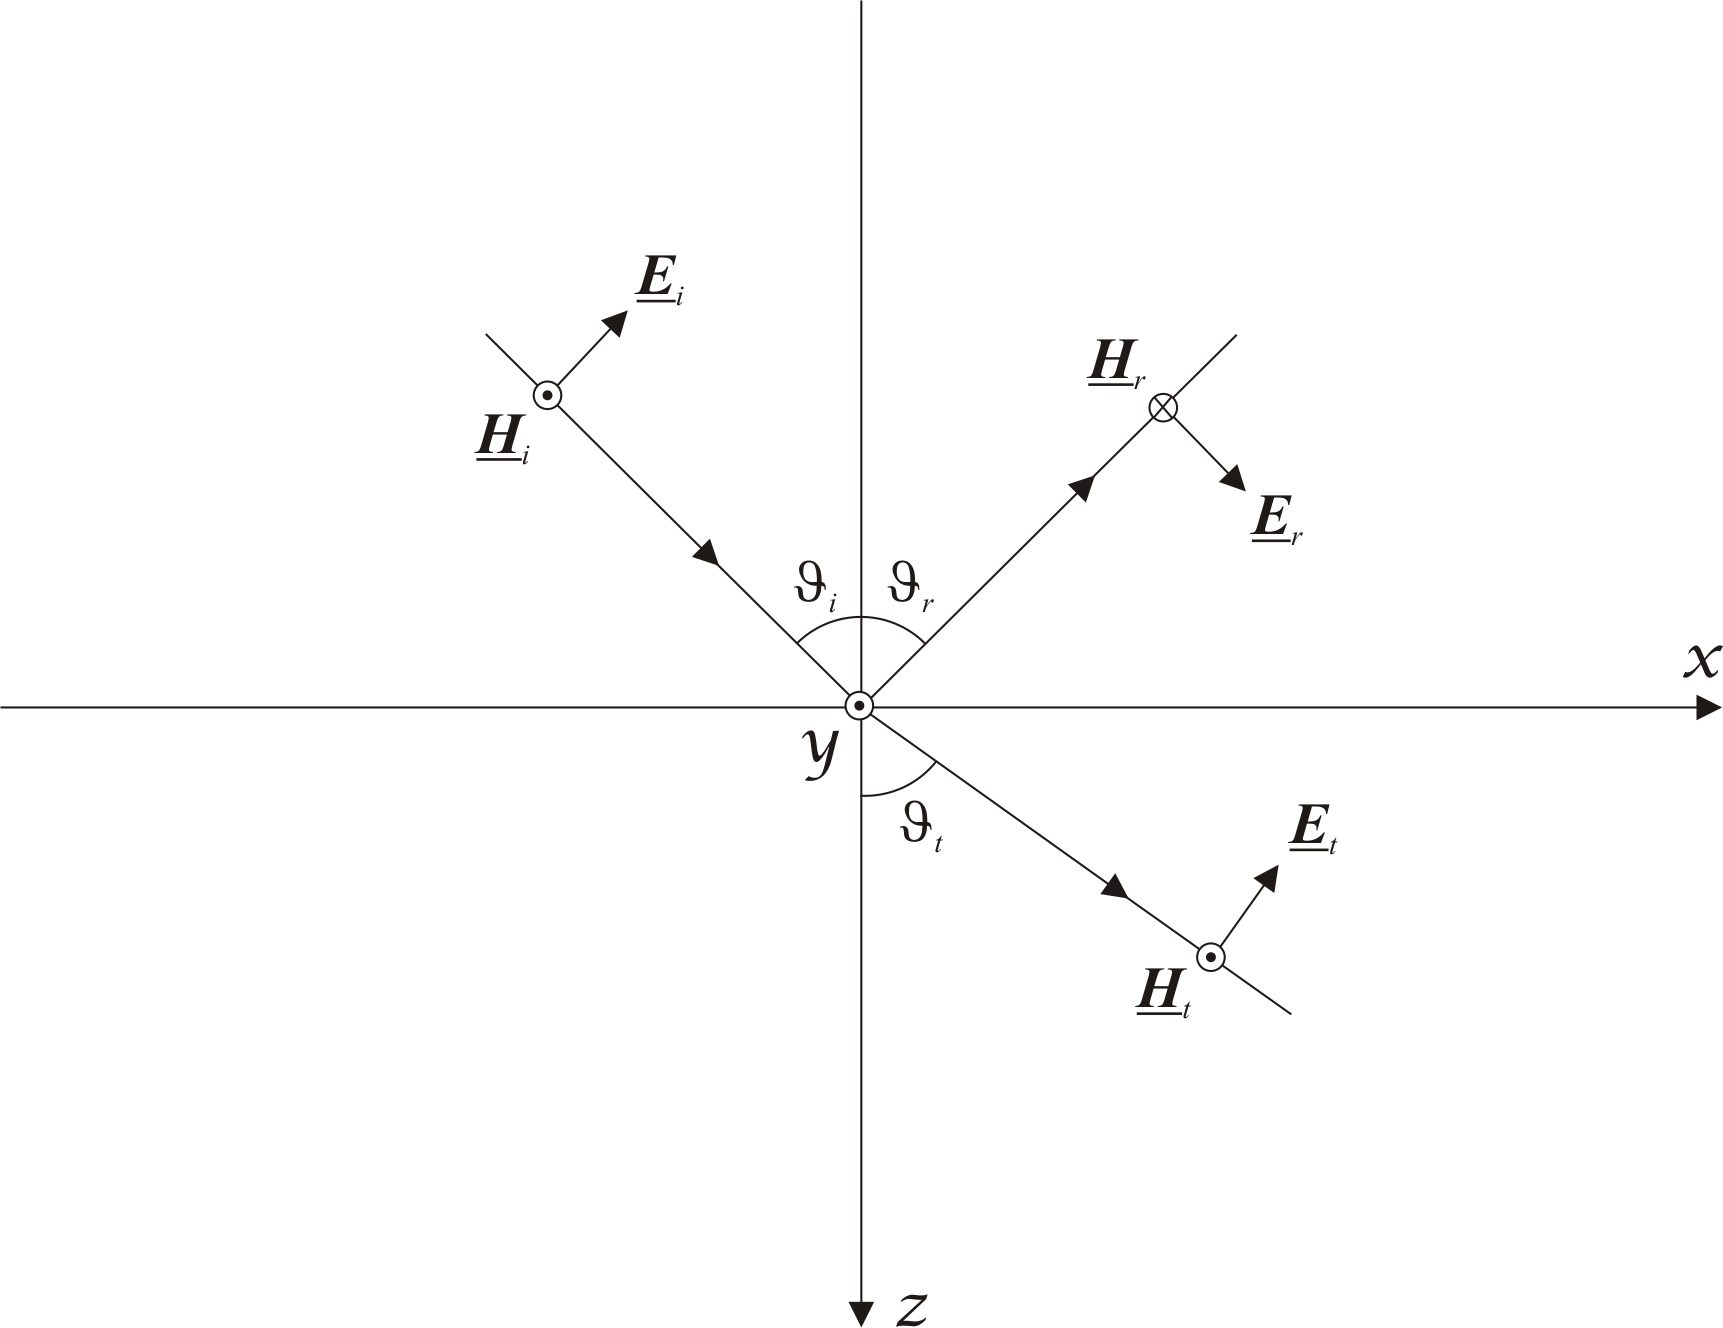
\includegraphics[width=11cm]{evlny_rovnobezna_polarizace.png}
	\caption{Rovnoběžná polarizace rovinné vlny. \cite{emp}}
	\label{obr:evlny_rovnobezna_polarizace}
\end{figure}
Odvození vztahů pro činitele odrazu a prostupu se nachází v~\cite[str. 95]{emp}. Pro výsledné vztahy platí v~tomto případě $\faz R_{\parallel} + 1 = \faz T_{\parallel}\frac{\cos\vartheta_{t}}{\cos\vartheta_{i}}$
\begin{equation}
	\faz R_{\parallel} = \frac{\faz E_{r0}}{\faz E_{i0}} = \frac{\faz Z_{2}\cos\vartheta_{t}-\faz Z_{1}\cos\vartheta_{i}}{\faz Z_{2}\cos\vartheta_{t}+\faz Z_{1}\cos\vartheta_{i}} = \frac{\faz Z_{2}\sqrt{1-(\faz k_{1}/\faz k_{2})^{2}\sin^{2}\vartheta_{i}}-\faz Z_{1}\cos\vartheta_{i}}{\faz Z_{2}\sqrt{1-(\faz k_{1}/\faz k_{2})^{2}\sin^{2}\vartheta_{i}}+\faz Z_{1}\cos\vartheta_{i}},
	\label{rce:evlny_cin_odrazu_rovnobezna}
\end{equation}
\begin{equation}
	\faz T_{\parallel} = \frac{\faz E_{t0}}{\faz E_{i0}} = \frac{2\faz Z_{2}\cos\vartheta_{i}}{\faz Z_{2}\cos\vartheta_{t}+\faz Z_{1}\cos\vartheta_{i}} = \frac{2\faz Z_{2}\cos\vartheta_{i}}{\faz Z_{2}\sqrt{1-(\faz k_{1}/\faz k_{2})^{2}\sin^{2}\vartheta_{i}}+\faz Z_{1}\cos\vartheta_{i}}.
	\label{rce:evlny_cin_prostupu_rovnobezna}
\end{equation}
Vztahy (\ref{rce:evlny_cin_odrazu_kolma}) až (\ref{rce:evlny_cin_prostupu_rovnobezna}) se také nazývají {\bf Fresnelovy rovnice}.

\subsection{Brewsterův polarizační úhel}
\subsubsection*{Situace u~kolmé polarizace dopadající vlny}
Úhel $\vartheta_{i}$ se označuje jako Brewsterův polarizační při splnění určitých podmínek. Pokud obecně polarizovaná elektromagnetická vlna dopadne na rozhraní pod tímto úhlem, tak odražená vlna bude mít pouze složku rovnoběžnou s~rovinou dopadu $xz$.

Odvození vychází ze vztahu pro $\faz R_{\perp}$ (\ref{rce:evlny_cin_odrazu_kolma}). Pokud bude platit $\faz Z_{2}\cos\vartheta_{i} = \faz Z_{1}\cos\vartheta_{t}$, tak činitel odrazu $\faz R_{\perp}$ vyjde nulový. To mimo jiné znamená, že se kolmo polarizovaná vlna neodráží a úplně celá prostupuje do druhého prostředí. Pomocí zákona lomu (\ref{rce:evlny_zakon_lomu}) a~vztahu $\cos\vartheta_{t} = \sqrt{1-\sin^{2}\vartheta_{t}}$ dostaneme
\begin{equation}
	\faz Z_{2}\cos\vartheta_{i} = \faz Z_{1}\sqrt{1-\bigg(\frac{\faz k_{1}}{\faz k_{2}}\bigg)^{2}\sin^{2}\vartheta_{i}}.
	\label{rce:evlny_brewster_kolma_odvozeni}
\end{equation}
Tento vztah (\ref{rce:evlny_brewster_kolma_odvozeni}) má řešení pro prostředí, kde platí $\mu_{1} \ne \mu_{2}$ a zároveň $\varepsilon_{1} = \varepsilon_{2}$. Výsledný výraz pro {\bf Brewsterův polarizační úhel} platí tedy pro tuto závislost materiálových konstant
\begin{equation}
	\sin\vartheta_{i\ BR} = \frac{1}{\sqrt{1+\frac{\mu_{1}}{\mu_{2}}}}.
	\label{rce:evlny_brewster_kolma}
\end{equation}

\subsubsection*{Rovnoběžná polarizace dopadající vlny}
Analogickým postupem jako v~předchozím případě vycházíme ze vztahu (\ref{rce:evlny_cin_odrazu_rovnobezna}) pro $\faz R_{\parallel}$. Zde se pro $\faz Z_{2}\cos\vartheta_{t} = \faz Z_{1}\cos\vartheta_{i}$ neodráží rovnoběžně polarizovaná vlna. Vztah Brewsterova polarizačního úhlu platí pro dielektrika ($\varepsilon_{1} \ne \varepsilon_{2}$), kde se po dopadu obecně polarizované vlny odráží složka polarizovaná kolmo na rovinu dopadu $xz$
\begin{equation}
	\sin\vartheta_{i\ BR} = \frac{1}{\sqrt{1+\frac{\varepsilon_{1}}{\varepsilon_{2}}}}.
	\label{rce:evlny_brewster_kolma}
\end{equation}
\newpage

\section{Vrstvené prostředí}
Při šíření elektromagentických vln v~reálných prostředích běžně dochází k~jevům na rozhraních. Ty jsou uvedeny v~podkapitole \ref{sec:evlny_rozhrani_dvou_prostredi}. V~praxi ale také může dojít k~přechodu vlny přes několik rozhraní za sebou, ať už se jedná o~požadovanou nebo nechtěnou funkci. Typicky se to týká šíření přes několik vrstev materiálu s~odlišnými parametry.

V~modelovém případě na obrázku \ref{obr:evlny_vrstvene_rada} se kolmo dopadající rovinná vlna $\vecfaz E_{i}$ částečně odráží a část proniká do prostředí popsaného vlnovou impedancí $\faz Z_{2}$. Zde může dále docházet k~mnohočetným odrazům. Prostupující vlna $\vecfaz E_{t}$ se nejprve odrazí od následujícího rozhraní $r_{23}$ jako $\vecfaz E_{tr}$. Poté může dojít na rozhraní $r_{12}$  k~průniku ($\vecfaz E_{trt}$) a dalšímu odrazu ($\vecfaz E_{trr}$) již původně odražené vlny. Tento proces se může opakovat dokud vlna v~daném prostředí nezanikne. Výsledná intenzita $\vecfaz E$ je pak dána součtem jednotlivých vln, které se vlivem odrazů a prostupů odráží. Vyjádření odražené vlny v~místě popsaném parametry s~indexem 1
\begin{equation}
	\vecfaz E_{1}^{-} = \vecfaz E_{r} + \vecfaz E_{trt} + \vecfaz E_{trrrt} + \cdots.
	\label{rce:evlny_vrstvene_rada1}
\end{equation}
Analogicky pro postupnou vlnu prostřední oblasti platí
\begin{equation}
	\vecfaz E_{2}^{+} = \vecfaz E_{t} + \vecfaz E_{trr} + \vecfaz E_{trrrr} + \cdots.
	\label{rce:evlny_vrstvene_rada2}
\end{equation}
\begin{figure}[!h]
	\centering
	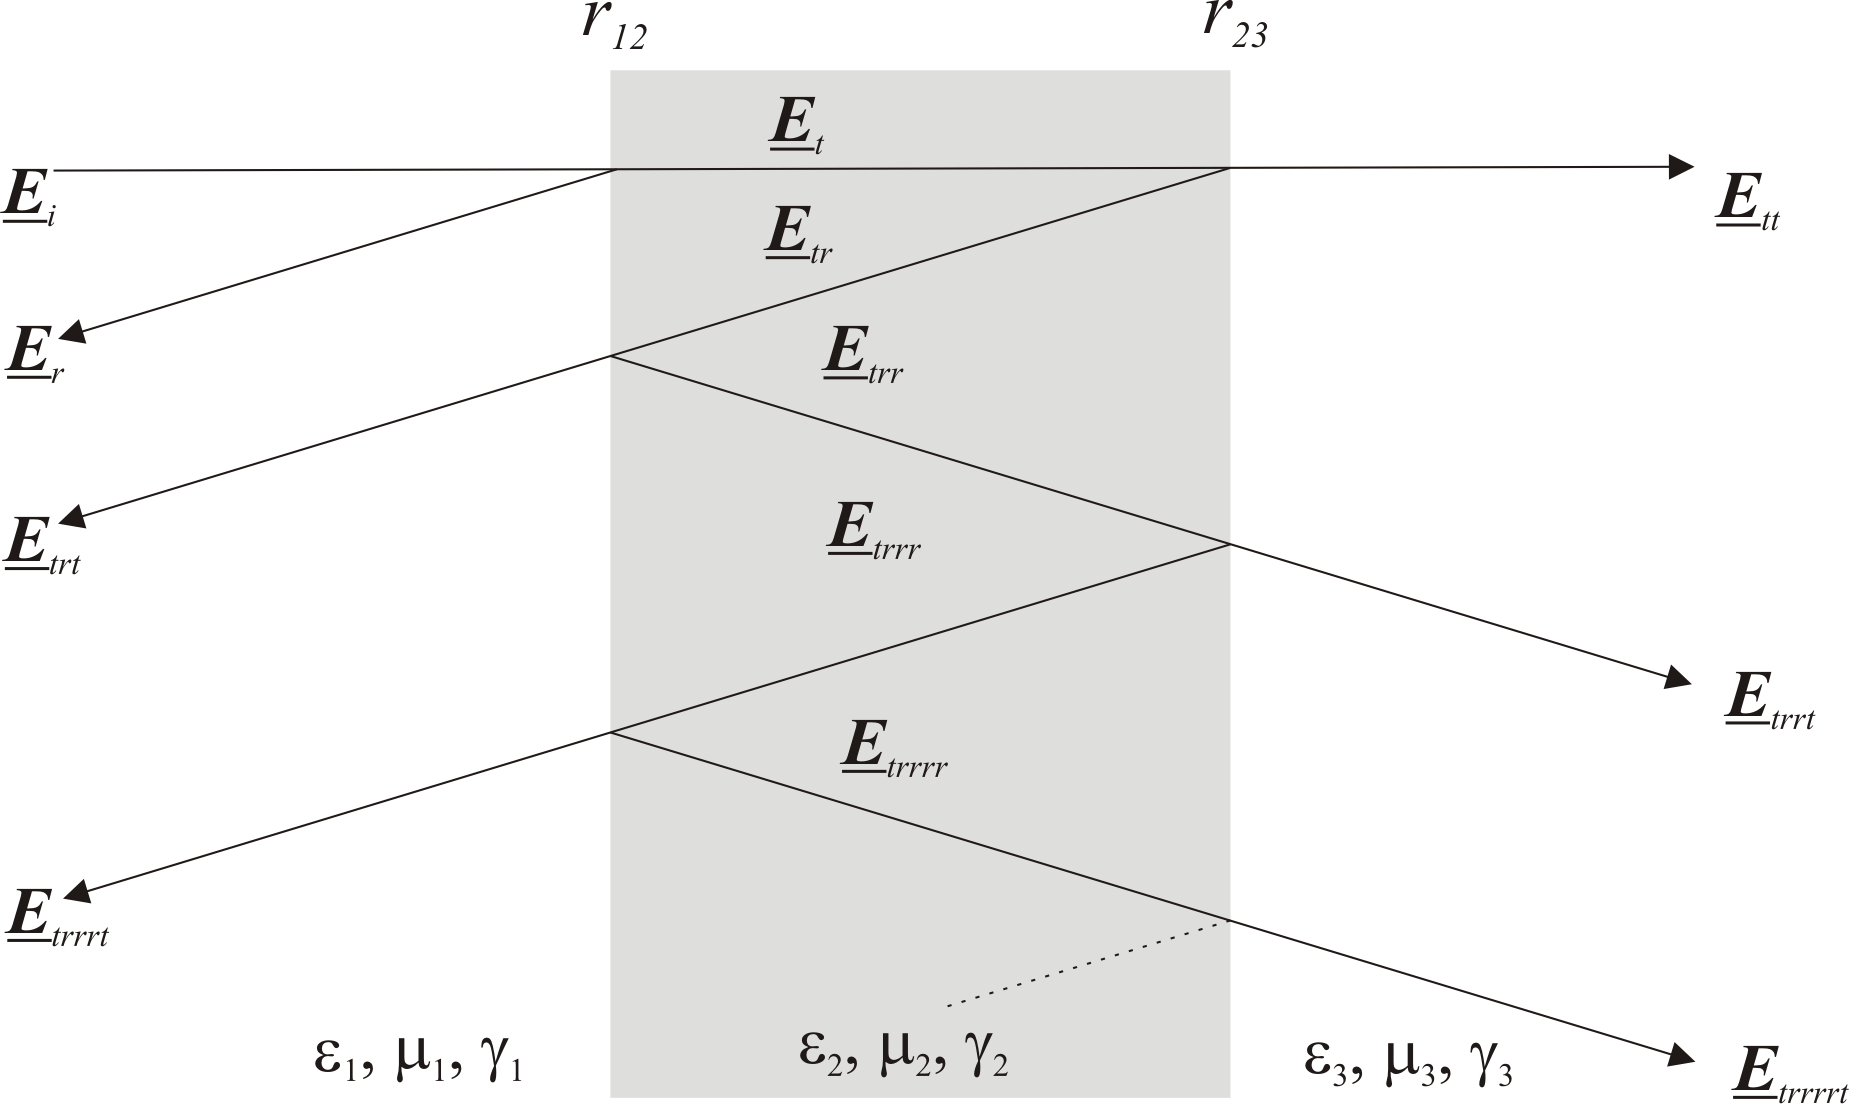
\includegraphics[width=12cm]{evlny_vrstvene_rada.png}
	\caption{Šíření elektromagnetických vln ve vrstveném prostředí. \cite{emp}}
	\label{obr:evlny_vrstvene_rada}
\end{figure}

\subsection{Metody řešení vln ve vrstveném prostředí}
Řešení chování elektromagnetické vlny vychází z~vyčíslení řad (\ref{rce:evlny_vrstvene_rada1}), (\ref{rce:evlny_vrstvene_rada2}), případně dalších. To je samo o~sobě ve většině případech velmi komplikované. Jednotlivé členy je pak potřeba sečíst s~ohledem na amplitudu a fázi. Pro další řešení existuje několik metod.
\begin{enumerate}
\item Součet vln stejného směru a vyjádření jedinou vlnou.
\item Maticová metoda.
\item Princip založený na transformaci vlnových impedancí.
\end{enumerate}

\subsubsection*{1. Součet vln stejného směru}
Postup této metody je blíže vysvětlen na příkladu v~\cite[str. 103 - 104]{emp}. V~každém prostředí, ve kterém se liší vlnová impedance $\faz Z$, se vyčíslí veškeré šířící se vlny. Například pro prostředí 1 na obrázku \ref{obr:evlny_vrstvene_rada} lze vyjádřit postupnou vlnu jako $\vecfaz E_{i}$ a odražená pak odpovídá výrazu (\ref{rce:evlny_vrstvene_rada1}). V~posledním prostředí uvažujeme pouze prostupující vlnu. Vyjádří se intenzita jak elektrického, tak i magnetického pole. Výsledné vlny se následně přizpůsobí podmínkám na rozhraní. Dostaneme soustavu, která bude mít počet rovnic závislý na počtu různých prostředí, přes které se elektromagnetická vlna šíří.

\begin{table}[!h]
\catcode`\-=12 
\begin{center}
  	\caption{Závislost počtu rovnic v~soustavě na vrstvách rozhraní.}
  	\label{tab:evlny_vrstvene_prostredi}
\begin{tabular}{|l|l|l|l|}
	\hline
	index & prostředí & počet rovnic & neznámých \\
	\hline
	0 & 2 & 2 & 3 \\
	1 & 3 & 4 & 5 \\
	2 & 4 & 6 & 7 \\
	\vdots & \vdots & \vdots & \vdots \\
	n & n+2 & 2n+2 & 2n+3 \\
	\hline
\end{tabular}
\end{center}
\end{table}

Pro tři prostředí (dle obrázku \ref{obr:evlny_vrstvene_rada}) dostaneme soustavu čtyř rovnic o~pěti neznámých. Aby ji bylo možné vyřešit, je potřeba znát alespoň jednu z~postupných nebo odražených vln. Ve většině případech je známá dopadající vlna $\vecfaz E_{i}$. 

\subsubsection*{2. Maticová metoda}
Je zřejmé, že první uvedená metoda bude s~nárůstem počtu vrstev čím dál více složitější. Postup další varianty řešení je opět rozebrán v~\cite[str. 105]{emp}. Tato metoda, jak už název napovídá, využívá matic. Pokud dopadají na rozhraní vlny z~obou stran podle obrázku \ref{obr:evlny_maticova_metoda1} je možné odvodit následující maticový tvar
\begin{equation}
\left[ \begin{array}{c}
\faz E_{1}^{+} \\
\faz E_{1}^{-} \\
\end{array} \right]
= 
\frac{1}{\faz T_ {12}}
\left[ \begin{array}{cc}
1 & \faz R_{12} \\
\faz R_{12} & 1 \\
\end{array} \right]
\cdot
\left[ \begin{array}{c}
\faz E_{2}^{+} \\
\faz E_{2}^{-} \\
\end{array} \right],
\label{rce:evlny_maticova_rozhrani}
\end{equation}
kde $\faz R_{12}$ představuje činitel odrazu a $\faz T_ {12}$ činitel prostupu při průchodu elektromagnetické vlny z~prostředí 1 do 2. 
\begin{figure}[!h]
	\centering
	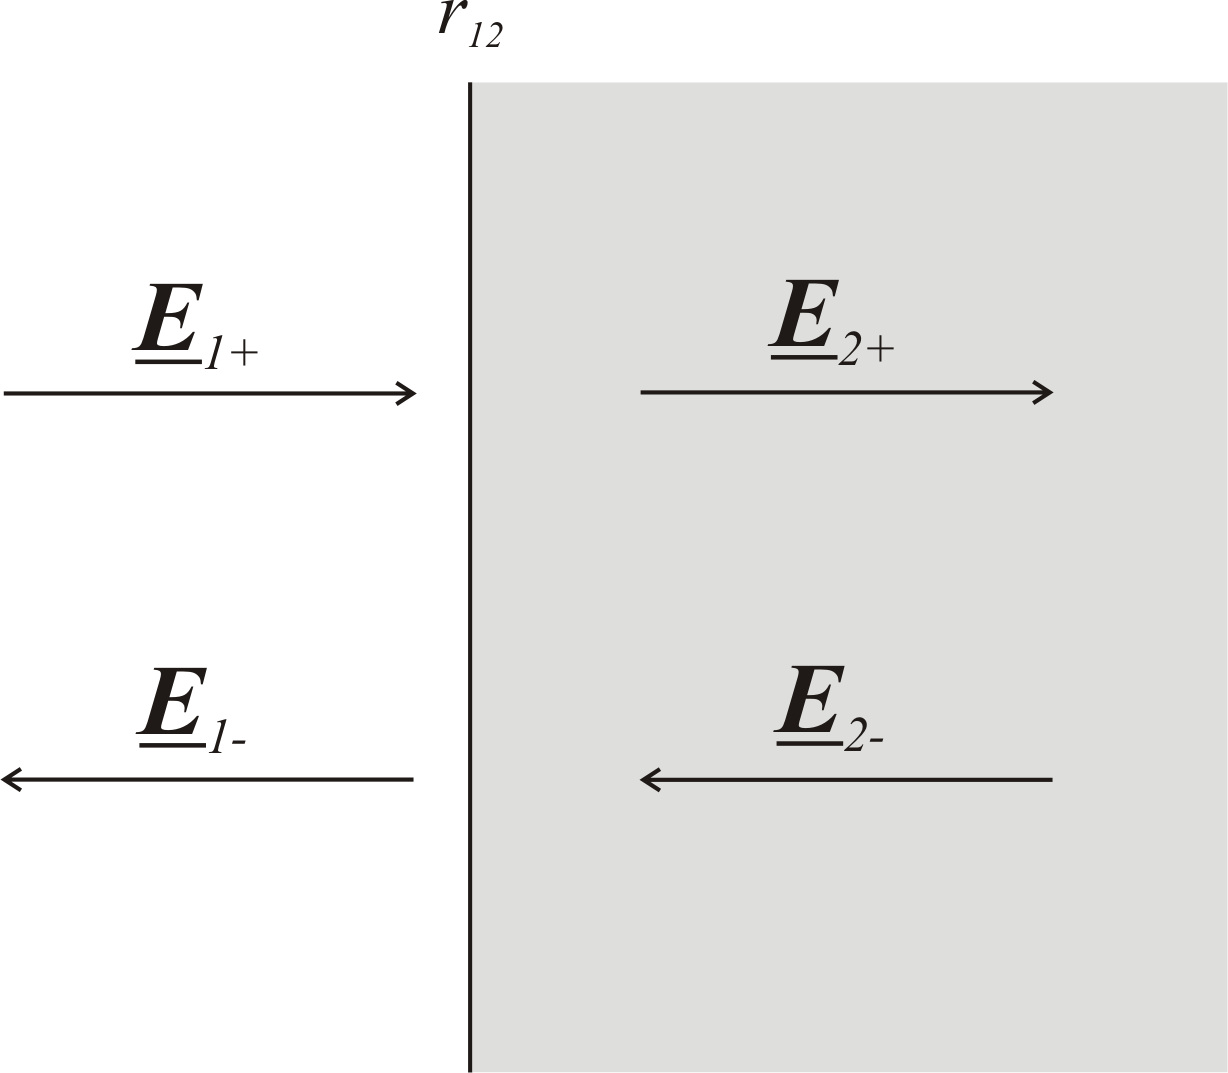
\includegraphics[width=5.5cm]{evlny_maticova_metoda1.png}
	\caption{Vlny dopadající na rozhraní z~obou stran. \cite{emp}}
	\label{obr:evlny_maticova_metoda1}
\end{figure}

Pokud bude vlna procházet vrstvou o~tloušťce $d$, ve které je popsána konstantou šíření $\faz k$, je opět možné podle situace na obrázku \ref{obr:evlny_maticova_metoda2} získat maticový zápis
\begin{equation}
\left[ \begin{array}{c}
\faz E_{2}^{+} \\
\faz E_{1}^{-} \\
\end{array} \right]
=
\left[ \begin{array}{cc}
\me^{\mj\faz k~d} & 0 \\
0 & \me^{-\mj\faz k~d} \\
\end{array} \right]
\cdot
\left[ \begin{array}{c}
\faz E_{3}^{+} \\
0 \\
\end{array} \right].
\label{rce:evlny_maticova_pruchod}
\end{equation}
\begin{figure}[!h]
	\centering
	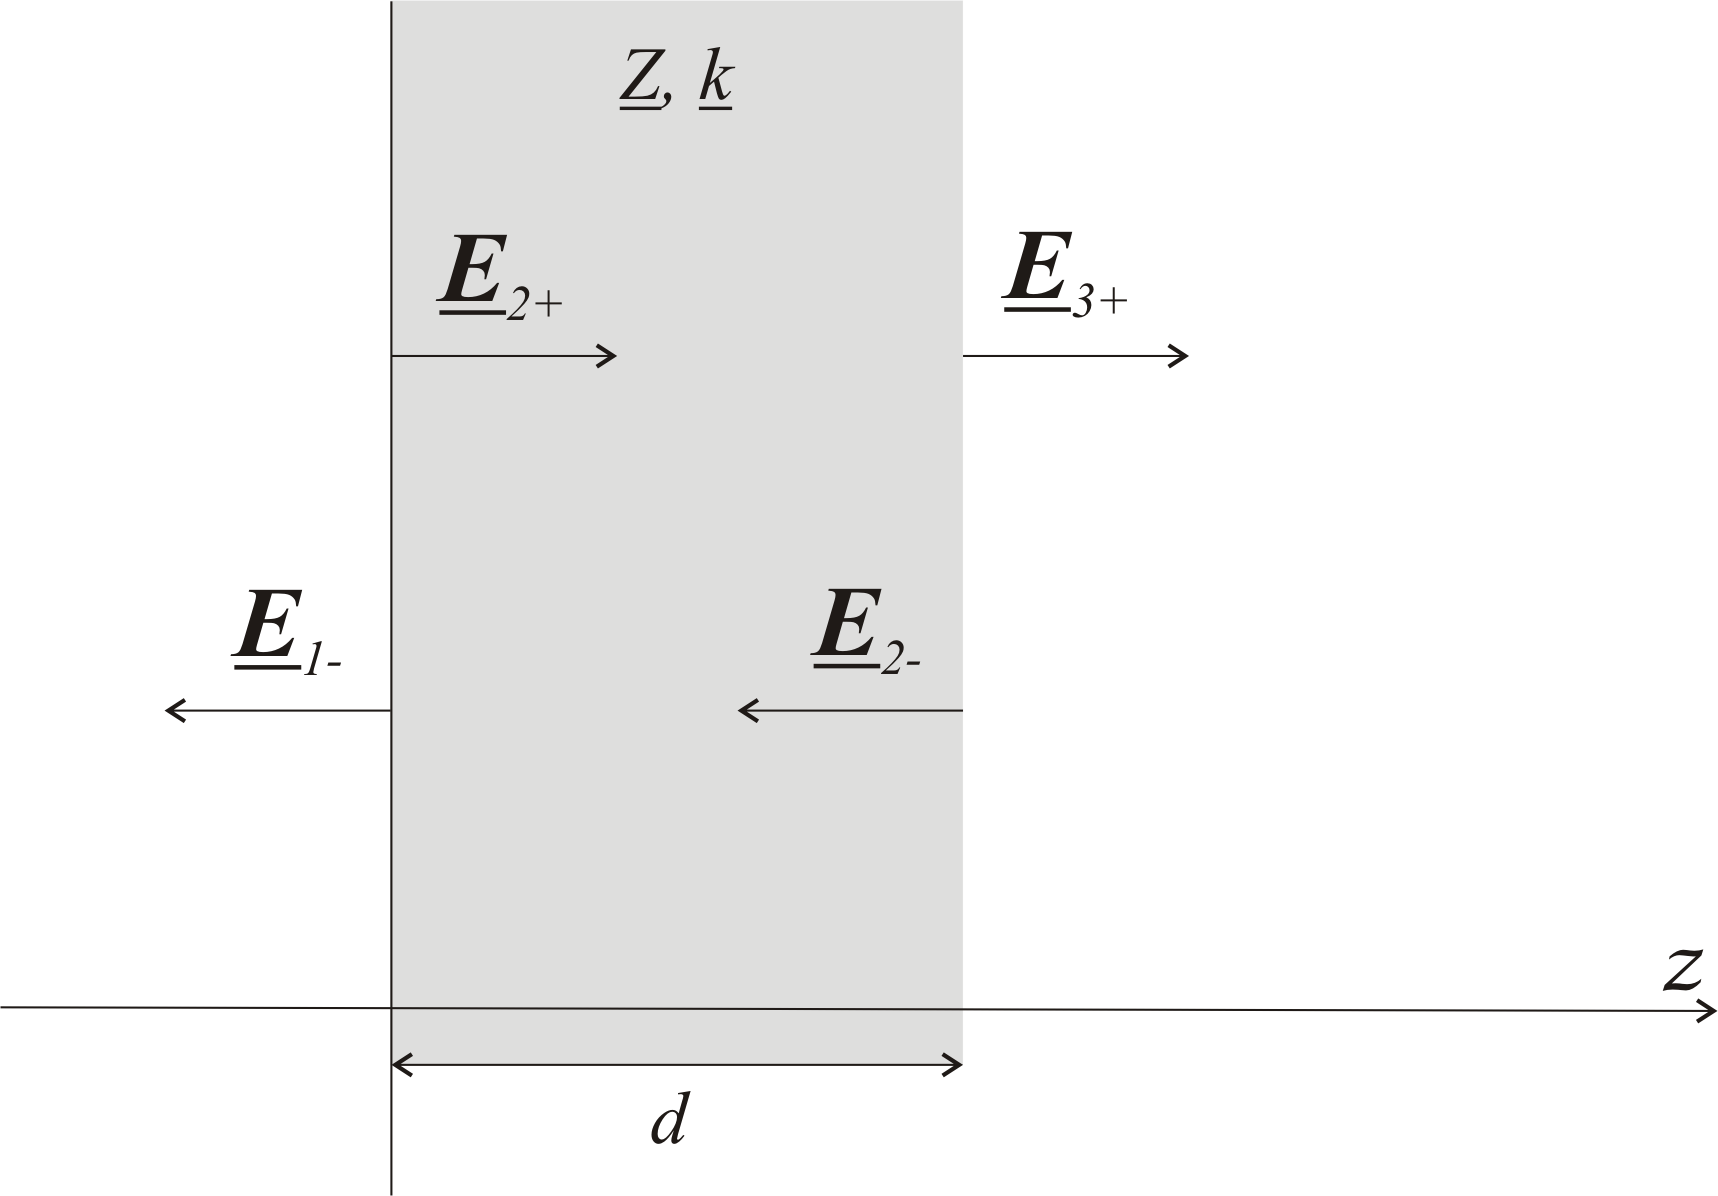
\includegraphics[width=8cm]{evlny_maticova_metoda2.png}
	\caption{Vlna procházející prostředím o~tloušťce $d$. \cite{emp}}
	\label{obr:evlny_maticova_metoda2}
\end{figure}

V~případě složité kombinace několika vrstev prostředí se využívá odvozených vztahů (\ref{rce:evlny_maticova_rozhrani}) a (\ref{rce:evlny_maticova_pruchod}) tak, že se postupně za sebou násobí takové matice, podle toho na jaké rozhraní elektromagnetická vlna dopadá a jakým prostředím prochází. Příklad šíření je uveden na obrázku \ref{obr:evlny_maticova_metoda3}. Vlna, šířící se z~prostředí 1 do prostředí 4, projde přes dvě oblasti o~tloušťce $d_{1}$, $d_{2}$ a tři rozhraní $r_{12}$, $r_{23}$ a $r_{34}$. Pro výslednou sestavu matic platí 
\begin{displaymath}
\left[ \begin{array}{c}
\faz E_{1}^{+} \\
\faz E_{1}^{-} \\
\end{array} \right]
=
\frac{1}{\faz T_ {12}}
\left[ \begin{array}{cc}
1 & \faz R_{12} \\
\faz R_{12} & 1 \\
\end{array} \right]
\cdot
\left[ \begin{array}{cc}
\me^{\mj\faz k_{2} d_{1}} & 0 \\
0 & \me^{-\mj\faz k_{2} d_{1}} \\
\end{array} \right]
\cdot
\frac{1}{\faz T_ {23}}
\left[ \begin{array}{cc}
1 & \faz R_{23} \\
\faz R_{23} & 1 \\
\end{array} \right]
\cdot
\end{displaymath}

\begin{equation}
\cdot
\left[ \begin{array}{cc}
\me^{\mj\faz k_{3} d_{2}} & 0 \\
0 & \me^{-\mj\faz k_{3} d_{2}} \\
\end{array} \right]
\cdot
\frac{1}{\faz T_ {34}}
\left[ \begin{array}{cc}
1 & \faz R_{34} \\
\faz R_{34} & 1 \\
\end{array} \right]
\cdot
\left[ \begin{array}{c}
\faz E_{4}^{+} \\
0 \\
\end{array} \right].
\end{equation} 
\begin{figure}[!h]
	\centering
	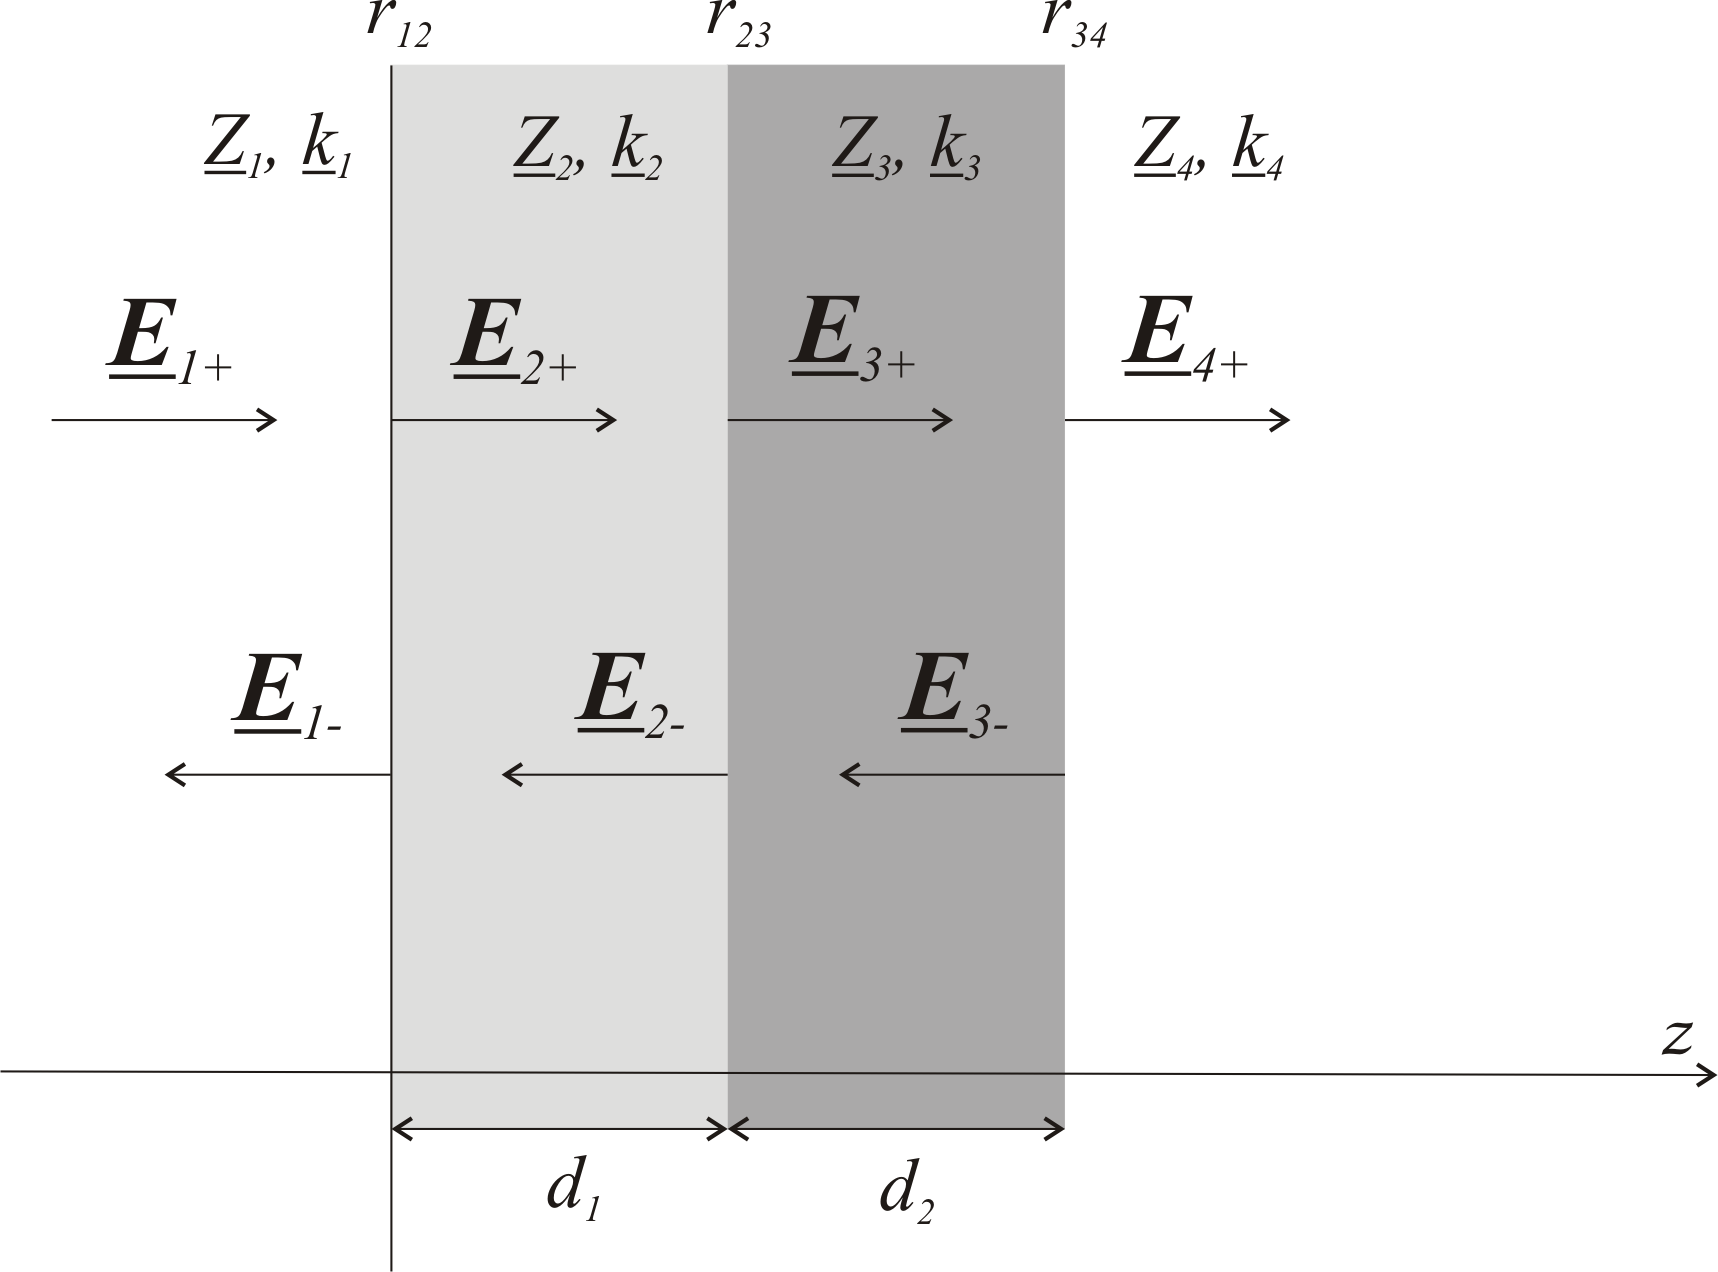
\includegraphics[width=8cm]{evlny_maticova_metoda3.png}
	\caption{Příklad vlny procházející přes dvě oblasti $d_{1}$ a $d_{2}$.}
	\label{obr:evlny_maticova_metoda3}
\end{figure}

\subsubsection*{3. Transformace vlnových impedancí}
Další možnost pro řešení vícevrstvých rozhraní vychází z~postupů, které se používají v~teorii vedení. Principem této metody je v~každém kroku výpočtu transformovat vlnovou impedanci posledního prostředí do místa rozhraní s~předcházející vrstvou. 
Odvození používaných vzorců se nachází v~\cite[str. 106]{emp}.
Pro situaci na obrázku \ref{obr:evlny_maticova_metoda3} bude prvním krokem transformace impedance $\faz Z_{3}$ a $\faz Z_{4}$ na rozhraní $r_{23}$ podle vztahu
\begin{equation}
	\faz Z_{c3}(r_{23}) = \faz Z_{3}\frac{\faz Z_{4}\cos(\faz k_{3}d_{2})+\mj\faz Z_{3}\sin(\faz k_{3}d_{2})}{\faz Z_{3}\cos(\faz k_{3}d_{2})+\mj\faz Z_{4}\sin(\faz k_{3}d_{2})}\unit{[\Omega]}.
	\label{rce:elvny_vrstvene_transformace1}
\end{equation}
V~dalším kroku se analogickým způsobem vypočtená impedance z~výrazu (\ref{rce:elvny_vrstvene_transformace1}) přepočte na rozhraní $r_{12}$
\begin{equation}
	\faz Z_{c2}(r_{12}) = \faz Z_{2}\frac{\faz Z_{c3}(r_{23})\cos(\faz k_{2}d_{1})+\mj\faz Z_{2}\sin(\faz k_{2}d_{1})}{\faz Z_{2}\cos(\faz k_{2}d_{1})+\mj\faz Z_{c3}(r_{23})\sin(\faz k_{2}d_{1})}\unit{[\Omega]}.
	\label{rce:elvny_vrstvene_transformace2}
\end{equation}
Nakonec je možné definovat činitele prostupu (\ref{rce:evlny_cin_prostupu}) a odrazu (\ref{rce:evlny_cin_odrazu}) na rozhraní $r_{12}$
\begin{equation}
	\faz R = \frac{\faz Z_{c2}(r_{12}) - \faz Z_{1}}{\faz Z_{1} + \faz Z_{c2}(r_{12})}
	\label{rce:elvny_vrstvene_transf_R},
\end{equation}
\begin{equation}
	\faz T = \frac{2\faz Z_{c2}(r_{12})}{\faz Z_{1} + \faz Z_{c2}(r_{12})}
	\label{rce:elvny_vrstvene_transf_T}.
\end{equation}
\newpage

\section{Vlnovody}
Během šíření vln ve volném prostředí od zdroje k~přijímací anténě dochází přirozeně k~rozptylu energie do prostoru. Anténou je tak zachycena pouze její část. To platí i pro směrové vysílací antény, pokud přenos probíhá na velké vzdálenosti. Pro zvýšení jeho efektivity je potřeba použít nějaké konstrukce, která umožňuje vedení energie.

To je možné zprostředkovat právě pomocí vlnovodů, jejichž nejběžnější provedení jsou na obrázku \ref{obr:evlny_vlnovody_konstrukce}. Vlnovody představují přípravek, ve kterém se elektromagnetická vlna šíří podélně ve směru osy $z$. V~příčném směru (tj. podle os $x$ a $y$) vzniká tzv. stojaté vlnění.
\begin{figure}[!h]
	\centering
	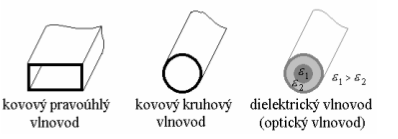
\includegraphics[width=7cm]{evlny_vlnovody_konstrukce.png}
	\caption{Nejběžnější konstrukce vlnovodů. \cite{emp}}
	\label{obr:evlny_vlnovody_konstrukce}
\end{figure}
Výhody vlnovodů jsou, kromě malých ztrát přenosu, v~nízké úrovni vyzařování do okolí  . Nevýhodou může být jejich cena a výroba pro velmi vysoké kmitočty. 

Další možnost pro přenos energie poskytují vedení, například dvouvodičnové, koaxiální nebo mikropáskové, které jsou popsané v~\cite{emp}.

\subsection{Klasifikace vln}
Vedené vlny lze rozlišit na několik druhů. Toto dělení se děje podle podélných složek pole, kterými jsou $\faz E_{z}$ a $\faz H_{z}$. V~případě vlnovodů se vnitřním prostorem šíří vlny typu TM a TE.

\subsubsection*{TEM vlny}
U~TEM, nebo-li transverzálně elektromagnetických vln jsou obě podélné složky pole nulové. Pro příčné složky, označené indexem $\perp$, platí dle \cite{emp} vztahy
\begin{displaymath}
	\nabla^{2}_{\perp} \vecfaz E_{\perp} = 0,
\end{displaymath}
\begin{displaymath}
	\nabla^{2}_{\perp} \vecfaz E_{\perp} = 0.
\end{displaymath}
Charakterem odpovídají tyto rovnice elektrostatickému poli, proto i rozložení pole pro TEM vlny bude obdobné.

\subsubsection*{TM vlny}
Transverzálně magnetické nebo také elektrické vlny mají nulovou složku magnetického pole $\faz H_{z}$. Složka elektrického pole $\faz E_{z}$ je nenulová. Řešení pole vychází z~vlnové rovnice ve tvaru
\begin{displaymath}
	\nabla^{2} \faz E_{z} + \faz k^{2}\faz E_{z} = 0,
\end{displaymath}
kde $\faz k$ představuje konstatnu šíření ve volném prostoru. Ta se skládá z~podélné $\faz k_z$ a příčné $\faz k_p$ konstanty šíření. Mezi sebou jsou vázány vztahem $\faz k^{2} = \faz k_z^{2} + \faz k_p^{2}$. Pro impedanci vlnovodu $\faz Z_{V}$ platí pro TM vlny vztah
\begin{displaymath}
   \faz Z_{V}^{TM} = \frac{\faz k_z}{\omega\varepsilon}\unit{[\Omega]}.
\end{displaymath}

\subsubsection*{TE vlny}
TE označuje vlny transverzálně elektrické. To jsou takové, které mají $\faz E_{z} = 0$. Příslušná vlnová rovnice má tvar
\begin{displaymath}
	\nabla^{2} \faz H_{z} + \faz k^{2}\faz H_{z} = 0.
\end{displaymath}
Impedance vlnovodu pro TE vlny je
\begin{displaymath}
	\faz Z_{V}^{TE} = \frac{\omega\mu}{\faz k_z}\unit{[\Omega]}.
\end{displaymath} 
\subsubsection*{EH a HE vlny}
Tento typ vln se vyskytuje ve vlnovodech složených z~několika dielektrik. Mají obě podélné složky pole nenulové a někdy se také označují jako vlny hybridní. Podle poměru $\frac{\faz E_z}{\faz H_z}$ se rozlišuje označení EH nebo HE.

\subsection{Parametry vlnovodů obdélníkových průřezů}
Tento typ vlnovodu patří k~nejběžněji používaným. 
Pro příčnou konstantu $k_p$ platí 
\begin{displaymath}
	k_p = \sqrt{\bigg(\frac{m\pi}{a}\bigg)^{2} + \bigg(\frac{n\pi}{b}\bigg)^{2}},
\end{displaymath}
kde $m, n = 1, 2, 3,\cdots$. Hodnoty $a$ a $b$ představují geometrii vlnovodu.

\subsection*{Mezní (kritická) frekvence}
Aby mohla být elektromagnetická vlna vedena vlnovodem, je potřeba, aby její kmitočet byl vyšší než mezní, který je definován
\begin{equation}
f_{m} = \frac{c}{2\pi\sqrt{\varepsilon_{r}\mu_{r}}}\cdot k_p = \frac{c}{2\sqrt{\varepsilon_{r}\mu_{r}}}\cdot \sqrt{\bigg(\frac{m}{a}\bigg)^{2} + \bigg(\frac{n}{b}\bigg)^{2}}\unit{[Hz]}. 
	\label{rce:evlny_vlnovody_mezni_frekvence}
\end{equation}
Tato hodnota je stejná jak pro TM, tak i pro TE vlny.
\subsection*{Mezní (kritická) vlnová délka}
Pro vedení vlny musí být vlnová délka menší než mezní, pro kterou platí
\begin{equation}
\lambda_{m} = \frac{c}{f_{m}} = \frac{2\sqrt{\varepsilon_{r}\mu_{r}}}{\sqrt{\big(\frac{m}{a}\big)^{2} + \big(\frac{n}{b}\big)^{2}}}\unit{[m]}. 
	\label{rce:evlny_vlnovody_mezni_vlnova_delka}
\end{equation}
Vztah je opět stejný pro TM a TE vlny.
\subsection*{Impedance vlnovodu}
Velikost impedance vlnovodu závisí na typu šířících se vln. V~případě transverzálně magnetických platí
\begin{displaymath}
	\faz Z_{V}^{TM} = \frac{\faz k_z}{\omega\varepsilon} = \frac{\sqrt{k^{2} - \big(\frac{m}{a}\big)^{2} - \big(\frac{n}{b}\big)^{2}}}{\omega\varepsilon}\unit{[\Omega]}
\end{displaymath}
a pro TE vlny náleží vztah
\begin{displaymath}
	\faz Z_{V}^{TE} = \frac{\omega\mu}{\faz k_z} = \frac{\omega\mu}{\sqrt{k^{2} - \big(\frac{m}{a}\big)^{2} - \big(\frac{n}{b}\big)^{2}}}\unit{[\Omega]}.
\end{displaymath}

\section{Dutinové rezonátory}
V~elektrotechnice se běžně používají systémy, založené na principu rezonance. Pro nízké frekvence je lze zrealizovat pomocí vhodné kombinace indukčnosti L, kapacity C a odporu R. Ve vysokofrekvenční oblasti tento přístup není možný a funkci těchto systémů plní dutinové rezonátory. 

Významnou skupinu představují rezonátory vytvořené z~vlnovodů, kterým se uzavře vstupní a výstupní brána. Obecně se jedná o~objem dielektrika libovolného tvaru, který je uzavřen dobře vodivým pláštěm. V~praxi se však upřednostňují rezonátory jednoduchých geometrických forem, například pravoúhlé (obrázek \ref{obr:evlny_rezonator}), cylindrické nebo toroidiální. 
\begin{figure}[!h]
	\centering
	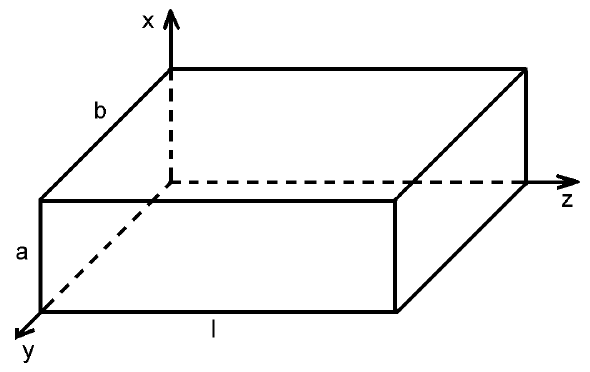
\includegraphics[width=7cm]{evlny_rezonator.png}
	\caption{Pravoúhlý dutinový rezonátor. \cite{tripak}}
	\label{obr:evlny_rezonator}
\end{figure}

Vzhledem ke skutečnosti, že rezonátory jsou uzavřený útvar, nedochází zde k~šíření vlny v~žádném směru. Mezi všemi stěnami se vyskytuje, podobně jako u~vlnovodů ve směru os $x$ a $y$, stojaté vlnění. U~rezonátorů tedy oproti vlnovodům existuje toto vlnění navíc i podél $z$-ové souřadnice. 

Analýzu jednotlivých typů rezonátorů je možné nalézt v~\cite{emp} nebo \cite{tripak}.

\subsection{Parametry rezonátorů}
Obdobně jako u~rezonančních systémů vytvořené z~R, L a C prvků, tak i u~dutinové rezonátory je možné charakterizovat několika parametry.
\subsection*{Rezonanční kmitočet}
\begin{displaymath}
	f_r = \frac{c}{2\sqrt{\varepsilon_r \mu_r}}\sqrt{\bigg(\frac{m}{a}\bigg)^{2} + \bigg(\frac{n}{b}\bigg)^{2} + \bigg(\frac{p}{d}\bigg)^{2}}\unit{[Hz]},
\end{displaymath}
kde $m, n, p = 1, 2, 3,\cdots$. Hodnoty $a$,$b$ a $d$ představují geometrii rezonátoru.
\subsection*{Kvalita (Jakost) rezonátoru}
Dalším důležitým parametrem rezonátoru se nazývá kvalita, případně jakost. Představuje míru ztrát energie za jednu periodu a je dána vztahem
\begin{displaymath}
	Q_0 = \omega_r \frac{W_{r}}{P},
\end{displaymath}
kde $\omega_r$ je úhlový rezonanční kmitočet, $W_r$ představuje nahromaděnou  energii a $P$ jsou výkonové ztráty v~rezonátoru.
\newpage